
\id{МРНТИ 52.13.15}{https://doi.org/10.58805/kazutb.v.4.25-549}

\begin{articleheader}
\sectionwithauthors{И.Н.Савич, Д.К. Бекбергенов, А.А.Зейнуллин, Р.К.Жанакова, А.С.Сейтенов, Д.Д.Мейрам}{МОДЕЛИРОВАНИЕ ГЕОМЕХАНИЧЕСКОЙ СИТУАЦИИ НАПРЯЖЕННОГО СОСТОЯНИЯ
МЕЖДУКАМЕРНЫХ ЦЕЛИКОВ ОСТАВЛЕННЫХ В ЗОНАХ ОБРУШЕНИЯ С МУЛЬДОЙ СДВИЖЕИЯ НА ПРИМЕРЕ ШАХТЫ «АННЕНСКАЯ» ВЖР}


{\bfseries \textsuperscript{1}И.Н.Савич, \textsuperscript{2}Д.К.
Бекбергенов\textsuperscript{\envelope }, \textsuperscript{3}А.А.Зейнуллин,
\textsuperscript{4}Р.К.Жанакова, \textsuperscript{5}А.С.Сейтенов, \textsuperscript{3,6}Д.Д.Мейрам}
\end{articleheader}

\begin{affiliation}

{\bfseries \textsuperscript{1}}НИТУ МИСИС, Москва, Россия,
{\bfseries \textsuperscript{2}}ИГД им.Д.А.Кунаева, Алматы, Казахстан,

{\bfseries \textsuperscript{3}}АО «Казахский университет технологии и
бизнеса им.К.Кулажанова, Астана. Казахстан,

\textsuperscript{4}Казахский автомобильно- дорожный института им. Л.Б.
Гончарова, Алматы, Казахстан,

\textsuperscript{5}Евразийский национальный университет им.
Л.Н.Гумилева, Астана, Казахстан,

{\bfseries \textsuperscript{6}}Карагандинского технического университета
им. А.Сагинова, Караганда, Казахстан

\raggedright{\bfseries \textsuperscript{\envelope }}Корреспондент-автор: kdbekbergen@mail.ru
\end{affiliation}

В данной статье приведены результаты исследований геомеханической
ситуации моделирования напряженно-деформированного состояния
междукамерных целиков, оставленных в условиях обрушенной зоны с мульдой
сдвижения на шахте «Анненская» ВЖР. Горнотехническая и геомеханическая
обстановка на шахтах ВЖР, и в том числе, на шахте «Анненская» весьма
сложная, где требуются исследования в натурных условиях и методом
моделирования с учетом НДС по оценке и обоснованию оставшихся запасов,
находящихся в сложных горнотехнических условиях в обрушенной зоне с
мульдой сдвижения залежей Жезказганского месторождения. В этой связи,
проведение научно-исследовательских работ обусловило необходимость
отработки оставшихся запасов в наклонных залежах под углом 20° при
разработке камерно-столбовой системой в указанных горнотехнических
условиях.

Статья является результатом научных исследований с ТОО Корпорация
«Казахмыс». выполненной в 2022 году под руководством Бекбергенова Д.К.

{\bfseries Ключевые слова:} моделирование, метод конечных элементов,
напряженно-деформированное состояние горных пород, междукамерные целики,
наклонные залежи, камерно-столбовая система, зона обрушения с мульдой
сдвижения, горизонтальное и вертикальное смещение, предел прочности
пород, шахта «Анненская» ВЖР

\begin{articleheader}

{\bfseries MODELING OF THE GEOMECHANICAL SITUATION OF THE STRESS STATE OF
INTERCHAMBER PILLARS LEFT IN THE COLLAPSING ZONES WITH A SHIFTING MOLD USING THE EXAMPLE OF THE ANNENSKAYA MINE OF THE EZhM}

{\bfseries \textsuperscript{1}I.N.Savich,
\textsuperscript{2}D.K.Bekbergenov\textsuperscript{\envelope },
\textsuperscript{3}А.А.Zeinullin, \textsuperscript{4}R.K.Zhanakova,
\textsuperscript{5}A.S.Seitenov, \textsuperscript{3,6}D.D.Meiram}
\end{articleheader}
\begin{affiliation}

{\bfseries \textsuperscript{1}}NUST MISIS, Moscow, Russia,
{\bfseries \textsuperscript{2}} IGD named after D.A. Kunaev, Almaty,
Kazakhstan,

{\bfseries \textsuperscript{3}}JSC Kazakh University of Technology and
Business named after K. Kulazhanov, Astana. Kazakhstan,

\textsuperscript{4} Kazakh Automobile and Road Institute named after.
L.B. Goncharova, Almaty, Kazakhstan,

\textsuperscript{5} Eurasian National University named after L.N.
Gumilyov, Astana, Kazakhstan,

\textsuperscript{6}Karaganda Technical University named after. A.
Saginova, Karaganda, Kazakhstan,

e-mail: kdbekbergen@mail.ru
\end{affiliation}

This article presents the results of studies of the geomechanical
situation of modeling the stress-strain state of inter-chamber pillars
left in the conditions of a collapsed zone with a displacement trough at
the Annenskaya mine of the EZhM. The mining and geomechanical situation
at the mines of the EZhM, including the Annenskaya mine, is very
complex, which requires research in natural conditions and by the
modeling method taking into account the stress-strain state to assess
and justify the remaining reserves located in difficult mining
conditions in the collapsed zone with a displacement trough of deposits
of the Zhezkazgan deposit. In this regard, the implementation of
research work necessitated the development of the remaining reserves in
inclined deposits at an angle of 20 ° when developing a room and pillar
system in the specified mining conditions.

The article is the result of scientific research with Kazakhmys
Corporation LLP. completed in 2022 under the leadership of Bekbergenov
D.K.

{\bfseries Keywords:} modeling, finite element method, stress-strain state
of rocks, inter-chamber pillars, inclined deposits, room-and-pillar
system, collapse zone with displacement trough, horizontal and vertical
displacement, ultimate strength of rocks, Annenskaya mine, EZhM

\begin{articleheader}

{\bfseries СТРЕССТІҢ ГЕОМЕХАНИКАЛЫҚ ЖАҒДАЙЫН МОДЕЛЬДЕУ АЙМАҚТАРДА ҚАЛҒАН ПАЛАМАТАРАЛЫҚ ПИЛЕРЛЕРДІҢ ЖАҒДАЙЫ ОРЫН АСЫРУ САУДАСЫНЫҢ КОЛЛАПСЫ: ШАХТА МЫСАЛЫ «АННЕНСКАЯ» ШЖК}

{\bfseries \textsuperscript{1}И.Н.Савич, \textsuperscript{2}Д.К.
Бекбергенов\textsuperscript{\envelope }, \textsuperscript{3}А.А.Зейнуллин,
\textsuperscript{4}Р.К.Жанакова, \textsuperscript{5}А.С.Сейтенов,
\textsuperscript{3,6}Д.Д.Мейрам}
\end{articleheader}
\begin{affiliation}

{\bfseries \textsuperscript{1}}НИТУ МИСИС, Москва, Россия,
{\bfseries \textsuperscript{2}}А. Қонаев атындағы тау-кен ісі институты,
Алматы, Қазақстан,

{\bfseries \textsuperscript{3}}АҚ «Қ.Құлажанов атындағы Қазақ технология
және бизнес университеті, Астана. Қазақстан,

\textsuperscript{4}Л.Б. Гончаров атындағы Қазақ автокөлік-жол институты,
Алматы, Қазақстан,

\textsuperscript{5}Л.Н.Гумилев атындағы Евразия ұлттық университеті,
Астана, Қазақстан,

\textsuperscript{6} Ә.Сағынов атындағы Қарағанды техникалық
университеті, Қарағанды, Қазақстан,

e-mail: kdbekbergen@mail.ru
\end{affiliation}

Бұл мақалада ШЖК Анненская кенішіндегі ығысу шұңқыры бар құлаған аймақ
жағдайында қалған камерааралық тіректердің кернеулі-деформациялық күйін
модельдеу геомеханикалық жағдайын зерттеу нәтижелері берілген. ШЖК
кеніштеріндегі, оның ішінде Анненская кенішіндегі тау-кен техникалық
және геомеханикалық жағдай өте күрделі. Табиғи жағдайларда және ҚҚС
ескере отырып модельдеу әдісімен зерттеу қажет, Жезқазған кен орнының
кен орындарының ығысу науасы бар қираған аймақта қиын өндіру жағдайында
орналасқан қалған қорларды бағалау және негіздеу. Осыған байланысты
ғылыми-зерттеу жұмыстары берілген тау-кен жағдайында бөлме-баған жүйесін
пайдалана отырып игерген кезде көлбеу кен орындарында қалған қорларды
20° бұрышпен игеруді қажет етті. Мақала «Қазақмыс Корпорациясы» ЖШС-мен
жүргізілген ғылыми зерттеулердің нәтижесі. Бекбергенов Д.К
жетекшілігімен 2022 жылы аяқталды.

{\bfseries Түйін сөздер:} модельдеу, шекті элементтер әдісі, тау
жыныстарының кернеулі-деформациялық күйі, камерааралық тіректер, көлбеу
шөгінділер, бөлме-бағаналық жүйе, ығысу науасы бар құлау аймағы,
көлденең және тік жылжу, тау жыныстарының беріктігі, Анненская шахтасы
ШЖК.
\begin{multicols}{2}

{\bfseries Введение.} С начала отработки запасов пологих залежей
Жезказганского месторождения практически ведется одной из самых
высокопроизводительных систем -- камерно-столбовой системой разработки с
использованием самоходного оборудования на дизельном ходу.

По горнотехническим и геомеханическим условиям Анненского района до 80\%
запасов руды сосредоточены в наклонных и перекрывающихся залежах, рудные
и породные массивы характеризуются повышенной трещиноватостью и
водонасыщенностью {[}1-5{]}.

Отработка Жезказганского месторождения в основном ведется
камерно-столбовой системой разработки наряду с другими системами
разработки для отработки наклонных участков, и ее доля составляет
порядка 85\%, а также освоена технология повторной отработки целиков из
открытого выработанного пространства с полевой подготовкой.

В пологих условиях Жезказганского месторождения традиционная
камерно-столбовая система разработки эффективно применяется на
меднорудных залежах с мощностью от 5 м до 18 м, где отработка панели
производится с оставлением МКЦ столбчатой формы по регулярной сетке 20 х
20 м (для пологих залежей) и 22 х 22 м (при наклонных залежах).

В соответствии с "Концепцией дальнейшей безопасной и эффективной
отработки запасов Жезказганского месторождения в усложнившихся
горно-геологических и горнотехнических условиях" {[}6,7{]}, с целью
дальнейшего обеспечения безопасных условий применения камерно-столбовой
системы разработки и снижения потерь в целиках, отработку запасов
пологих залежей необходимо производить в две стадии: I стадия - выемка
камерных запасов; II стадия - выемка целиков с обрушением налегающей
толщи в отступающем порядке.

По данным ПО «Жезказганцветмет распределение запасов Анненского района
по глубине залегания и мощности, основная часть (78,5\%) запасов
сконцентрирована на горизонтах от +90 м до --90 м (глубина залегания
330- 510 м). Ниже залегают всего 8,5\% запасов, а на верхних горизонтах
-- 19\%. Наиболее продуктивными (мощными и богатыми) являются залежи на
горизонтах от +90 м до --90 м. Геомеханические процессы, протекающие на
Жезказганском месторождении (разрушение МКЦ, сдвижение горных пород,
обрушение налегающей толщи с образованием провалов в земную поверхность,
с техногенными землетрясениями) не есть что-то, присущее только
Жезказгану, такие же процессы на всех рудниках, где в подобных
горно-геологических условиях применяют камерно-столбовую систему
разработки. При всех преимуществах, основными недостатками
камерно-столбовой системы разработки являются значительные потери руды
от 30\% до 40\%, а также накапливающиеся объемы пустот, которые приводят
к осложнению технологии очистной выемки, саморазрушению целиков

Основные трудности возникают в прогнозе поведения массива при извлечении
целиков, установлении допустимых границ и рационального способа
погашения выработанного пространства и порядка повторной разработки.
Основой для такого прогноза является анализ полей напряжений и смещений
в массиве горных пород, как в процессе первичной разработки, так и их
изменений в ходе повторной разработки.

Изучение напряженного состояния массивов горных пород рядом авторов
проводилось в Жезказгане методом разгрузки. Было установлено, что поле
напряжений в массиве не стационарно, а изменяется во времени,
анизотропно (в каждой точке горизонтальные напряжения не равны) и
неоднородно, т.к. изменяется от точки к точке. Установлено, что в
Жезказгане максимальное горизонтальное напряжение изменяется от 97 до 12
МПа, т.е. более чем в 8 раз; максимальные горизонтальные напряжения
субмеридиальные, минимальные - субширотного простирания.

Выемка целиков из открытого выработанного пространства требует строгого
соблюдения технологии выемки МКЦ в устойчивом выработанном пространстве
и запаса их прочности не менее 1,2 ÷ 1,5 с постоянным мониторингом
состояния выработанного пространства с использованием региональной
радиотелеметрической системы контроля сейсмических событий в режиме
реального времени {[}8-10{]}.

Выемка целиков через полевые выработки не требует повышенной
устойчивости выработанного пространства. При данной технологии
предусматривается отбойка руды из целика в зажиме обрушенных пород,
заполнение камер породами кровли предусматривается отрезка целиков по
верхнему основанию путем взрывания скважин, пробуренных через тело
целика в кровлю на высоту 1,5 ÷ 2,0 м . Недостатком этого способа, при
повторной отработке является большой объем горно-подготовительных работ
до 90 м³/1000 т, и низкий уровень показателей извлечения: повышенные
потери - до 45\%, разубоживание руды до 25\%.

При отработке рудных залежей, их мощность и площадь оказывают
существенное влияние на характер и величину сдвижения налегающих горных
пород.

Общий объем образованных пустот по информации технического отдела ВЖР,
на 01.01.2023 года составил: 85903,2 тыс. м³ (100\%), в т.ч. по шх.
Анненская -11744,3 тыс. м³. Из них 2015,1 тыс. м³ ослабленные, 1445,8
тыс. м³ неустойчивые.

К ослабленным участкам по шахте «Анненская» относятся старые блоки
15-15юг, 22, 23-24 и 54, а также не устойчивые панели П-54 (частично
обрушенные) и П-89бис.

Исходя из Заключения по анализу инцидента локального обрушения выработки
на шахте 42 горизонта 315 ВЖР с выходом на поверхность отмечено, что
локальное обрушение произошло 9 сентября 2020 года без сейсмического
проявления горного давления на участке по штреку 26 залежи Кр. 9 - II --
III с выходом на поверхность и расширением границ обрушения на
поверхности первые трое суток до 2 ÷ 3 м. При этом, площадь обрушения
составляет 140 х 100 м и повреждены водовод и коллекторные коммуникации
на поверхности, расположенные в пределах «Коридора». Причиной обрушения
по данному участку также является отрицательное влияние
производственного процесса доработки оставшихся запасов из целиков с
повторной отработкой при камерно-столбовой системе разработки.

Необходимо отметить, что горнотехническая и геомеханическая обстановка
на шахтах ВЖР и в том числе, на шахте «Анненская» весьма сложная, где
требуются исследования в натурных условиях и методом моделирования с
учетом НДС по оценке и обоснованию оставшихся запасов, находящихся в
обрушенной зоне с сейсмической активностью в условиях мульды сдвижения
залежей Жезказганского месторождения.

{\bfseries Материалы и методы.} Моделирование геомеханической ситуации
методом конечных элементов напряженно-деформированного состояния МКЦ в
наклонных залежах под углом 20° при повторной отработке запасов руд из
МКЦ, оставленных в условиях обрушенной зоны с мульдой сдвижения на
примере шахты «Анненская» ВЖР.

Расчет НДС оставленных междукамерных целиков (МКЦ) при камерно-столбовой
системе разработки реализован с применением метода конечных элементов в
программе RS Examine2D. Данная программа двухмерного моделирования
методом граничных элементов напряженно-деформированного состояния
массива при подземной разработке в упругой постановке. Программа
является интерактивной и простой в использовании, идеально подходит для
осуществления быстрого параметрического анализа, предварительного
проектирования, а также в качестве обучающего средства численному
анализу напряжений в геотехнических задачах.

Для компановки задачи напряженно-деформированного состояния МКЦ
необходимо создать схематичную модель контура МКЦ в целом с проектными
размерами параметров. Данная идея дает возможность увидеть состояния
наряду с ортогональным и изометрическим стилями, представления проекций
в целом системы разработки, в 3D AutoCAD создавая реалистичный стиль
представления проекций объекта (рисунок 1). На рисунках 2 и 3
представлены соответственно схема модели из объемных конечных элементов
(КЭ) с выделенным наклонным участком блока и схема расположения целиков
в блоке согласно камерно-столбовой системе разработки в условиях
наклонных залежей под углом 20\textsuperscript{0}.
\end{multicols}

\begin{figure}[H]
	\centering
	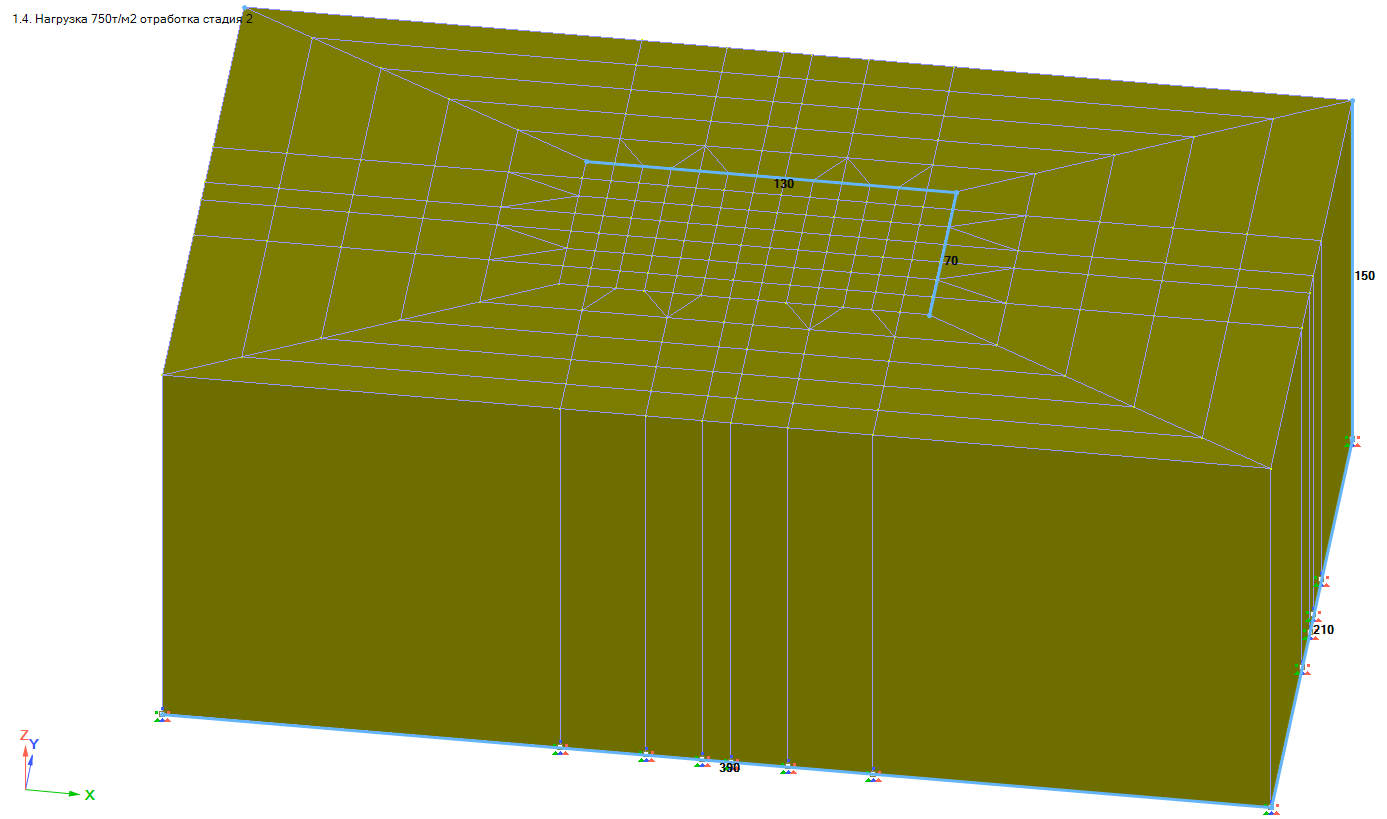
\includegraphics[width=0.6\textwidth]{media/gor/image6}
	\caption*{Рис. 1 - Расчетная модель с параметрами блока}
\end{figure}



\begin{figure}[H]
	\centering
	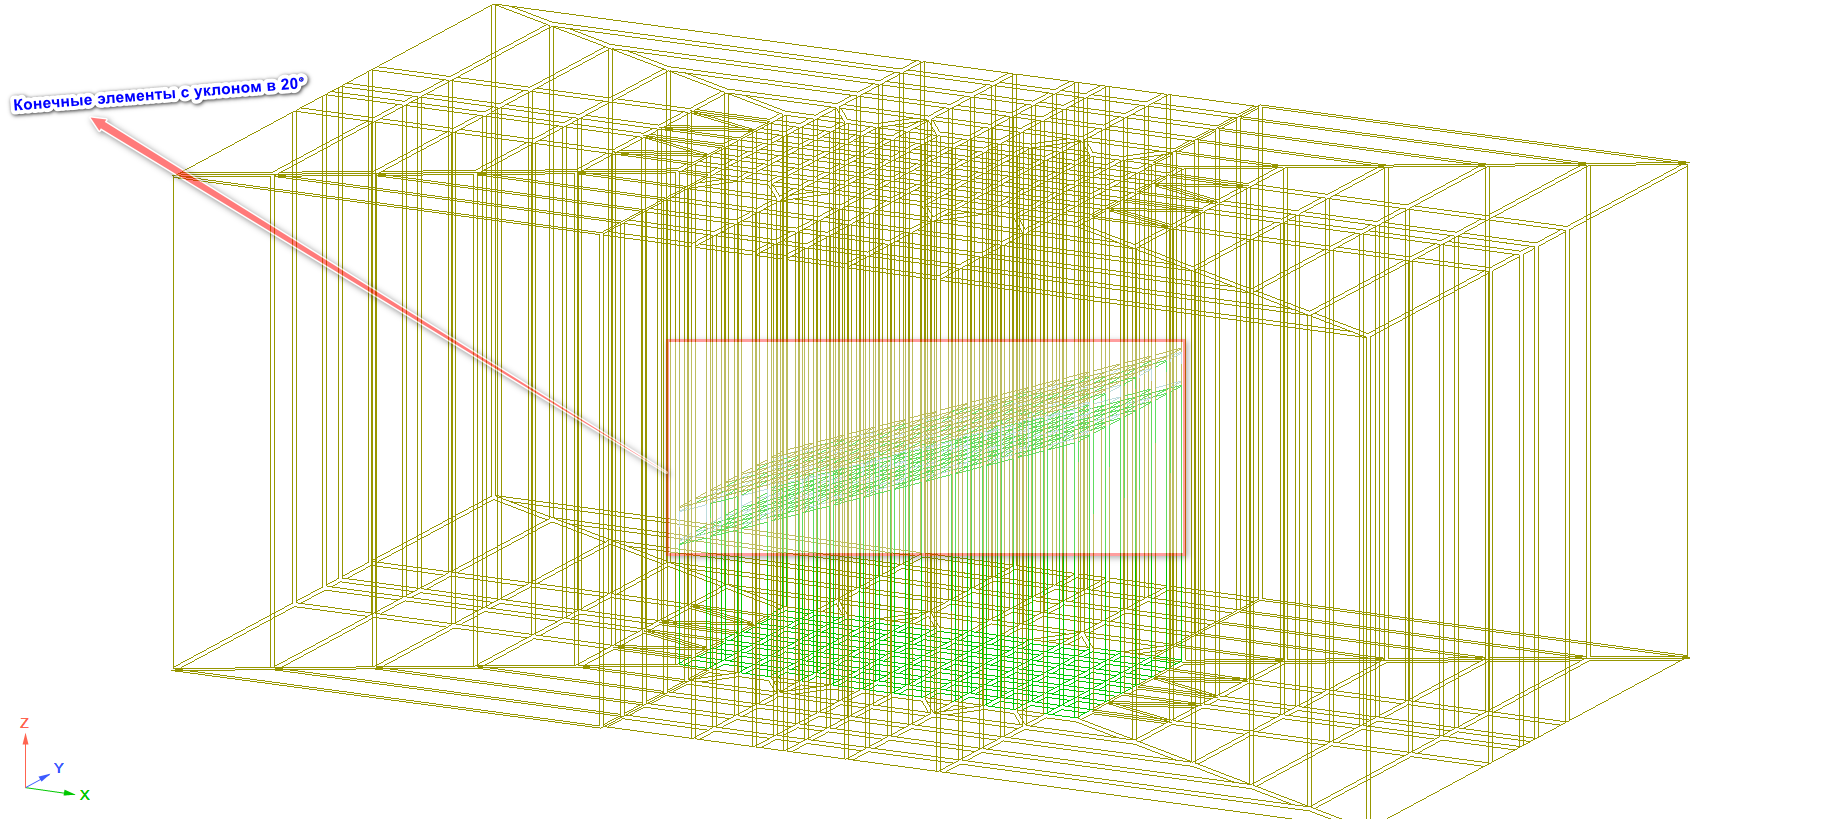
\includegraphics[width=0.8\textwidth]{media/gor/image7}
	\caption*{Рис. 2 -- Схема модели из объемных конечных элементов (КЭ) с
	выделенным наклонным участком блока}
\end{figure}



\begin{figure}[H]
	\centering
	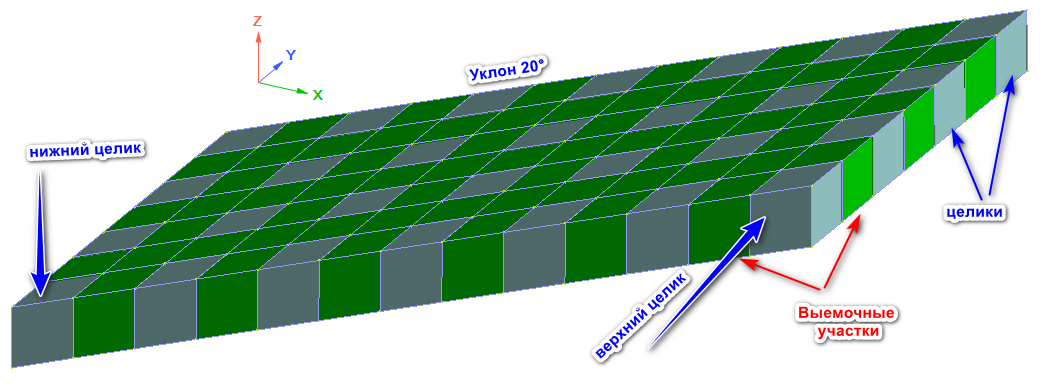
\includegraphics[width=0.8\textwidth]{media/gor/image8}
	\caption*{Рис. 3 - Схема расположения целиков в блоке согласно
	камерно-столбовой системе разработки в условиях наклонных залежей под
	углом 20\textsuperscript{0}}
\end{figure}


\begin{multicols}{2}

Пространственная схематическая модель представлена в форме куба, где
интересующие исследуемые участки расчетной образуют единую систему.
Схематическая модель состоит из 688 узлов и 413 объемных КЭ.
Геометрические размеры расчетной КЭ модели составляют 390х210х150 в
метрах. Размеры рассчитываемого блока 120х70х150 в метрах, где
отрабатываемая часть рудного массива наклонная с уклоном 20°, целики
которого приняты с размерами 10х10х10 м, с шагом по 10м представленных
на рисунках 2 и 3, где отражены общий вид с размерами расчетной модели.

Для серого рудного песчаника установлена закономерность изменения
прочности при одноосном сжатии с ростом глубины разработки, и в
диапазоне глубин 100÷400 м прочность серого рудного песчаника
увеличивается от 140 до 245 МПа, то есть в 1,7 раза, а также влияние
зоны выветривания прослеживается до глубины 150 м {[}11,12{]}.

Удельный вес вмещающих пород колеблется в пределах 2,5÷2,6 т/м\^{}3, руд
(в зависимости от содержания полезного компонента -- в пределах 2,55÷2,8
т/м³).

Наличие природной трещиноватости приводит к снижению прочности массива
горных пород. Величина коэффициента структурного ослабления w,
представляющего собой отношение прочности массива к прочности образца
зависит от размера структурного блока - a, высоты обнажения целика (h =
8-10 м) и диаметра целика (d = 10-12 м), и колеблется в пределах
0,3÷0,7.

В качестве входных параметров для материалов КЭ приняты
физико-механические характеристики пород, представленные в отчетах по
Анненскому рудному полю Жезказганского месторождения (таблица 1).

Представленные расчетные модели являются основанием для предстоящих
работ по исследованию стадийности и порядка отработки запасов из МКЦ при
повторной добыче отработанной камерно-столбовой системой, а также по
определению устойчивости подземных геомеханических конструкций МКЦ при
отработке запасов наклонных и крутопадающих блоков при камерно-столбовой
системе разработки с учетом изменения мощности рудных тел и способствуют
основой при отработке запасов из целиков и в зоне обрушений, большинство
из которых локализуется на перекрывающихся залежах.
\end{multicols}


\begin{table}[H]
\caption*{Таблица 1 - Физико-механические свойства руд и вмещающих пород Жезказганского месторождения}
\centering
\resizebox{\textwidth}{!}{%
\begin{tabular}{|c|cc|c|c|c|c|}
\hline
\multirow{2}{*}{Тип породы} &
  \multicolumn{2}{c|}{\begin{tabular}[c]{@{}c@{}}Предел прочности,\\   МПа\end{tabular}} &
  \multirow{2}{*}{\begin{tabular}[c]{@{}c@{}}Сцепле-ние,\\   МПа\end{tabular}} &
  \multirow{2}{*}{\begin{tabular}[c]{@{}c@{}}Угол \\ внутреннего\\   трения, град\end{tabular}} &
  \multirow{2}{*}{\begin{tabular}[c]{@{}c@{}}Модуль\\  упругости,\\  МПа\end{tabular}} &
  \multirow{2}{*}{\begin{tabular}[c]{@{}c@{}}Коэффициент\\   Пуассона, \\ доли единиц\end{tabular}} \\ \cline{2-3}
  & & & & & & \\
                         & \multicolumn{1}{c|}{на сжатие} & на растяжение &         &    &           &           \\ \hline
Медная руда              & \multicolumn{1}{c|}{140-230}   & 10 – 18       & 25 – 30 & 35 & 3,2 – 4,5 & 0,20-0,22 \\ \hline
\begin{tabular}[c]{@{}c@{}}Медно-свинцовая\\ руда\end{tabular}     & \multicolumn{1}{c|}{160-240}   & 10 - 18       & 30 - 34 & 35 & 5,0 – 6,5 & 0,18-0,21 \\ \hline
\begin{tabular}[c]{@{}c@{}}Серый безрудный\\ песчаник\end{tabular}  & \multicolumn{1}{c|}{160-245}   & 8 - 11        & 25 - 34 & 35 & 4,5 – 6,5 & 0,18-0,22 \\ \hline
Красный песчаник         & \multicolumn{1}{c|}{80-120}    & 2 – 4         & 20 – 25 & 30 & 3,9 – 4,2 & 0,20-0,22 \\ \hline
Красный алевролит        & \multicolumn{1}{c|}{30-60}     & 2 – 4         & 18 – 20 & 30 & 3,2 – 4,0 & 0,22-0,25 \\ \hline
\end{tabular}%
}
\end{table}

\begin{figure}[H]
	\centering
	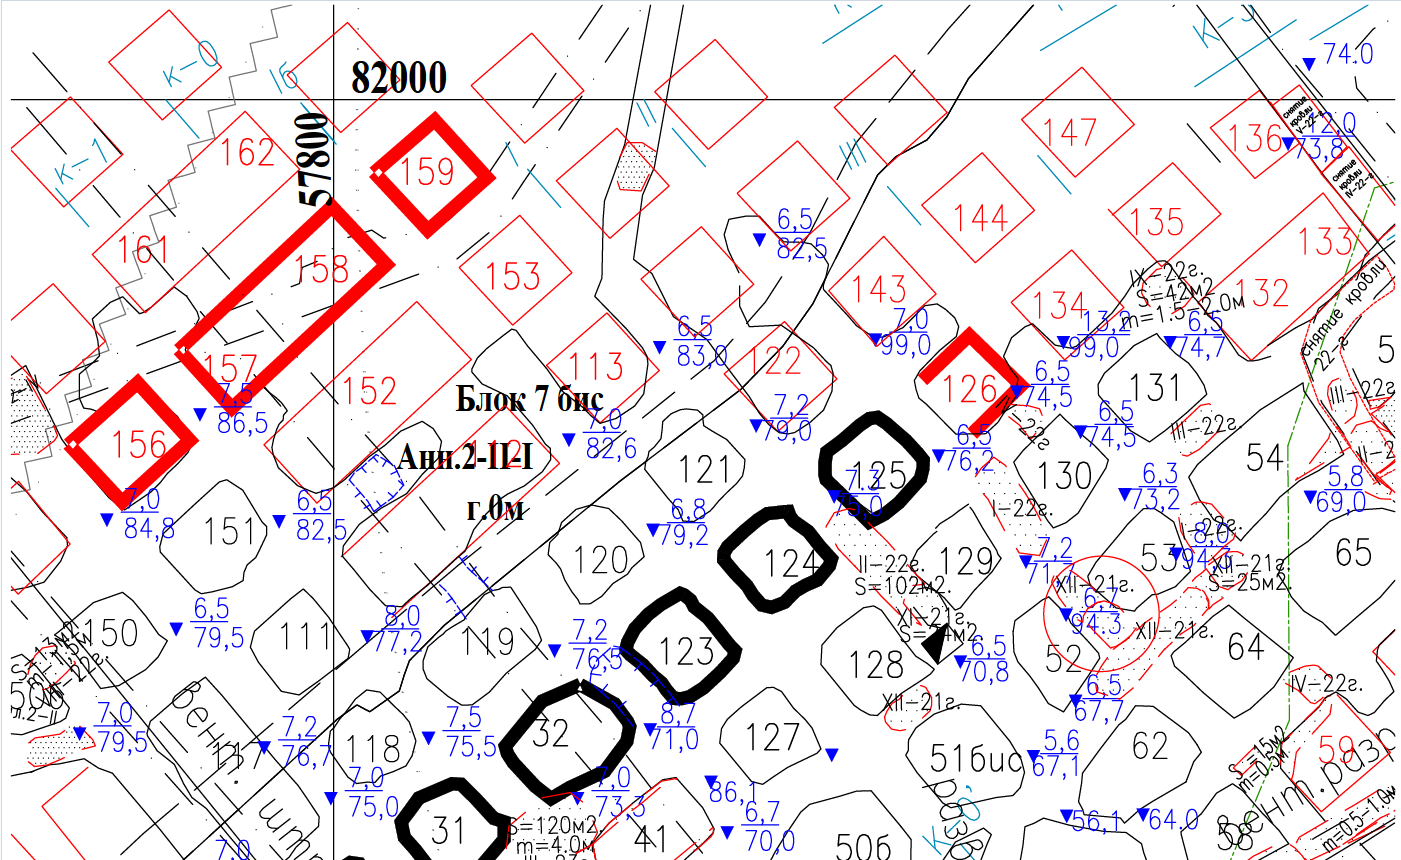
\includegraphics[width=0.6\textwidth]{media/gor/image9}
	\caption*{Рис. 4 - Расположение ряда целиков по блоку 7 бис Анн.2-II-I для
	исследования НДС}
\end{figure}

\begin{multicols}{2}
{\bfseries Результаты и обсуждение.} Расчетный анализ геомеханической
ситуации напряженно-деформированного состояния МКЦ в очистном
пространстве камерно-столбовой системой оставленного в условиях
обрушенной зоны с мульдой сдвижения, на примере блока 7 бис Анн.2-II-I
шахты «Анненская» ВЖР с применением метода конечных элементов.

Согласно отработки оставшихся запасов руд из МКЦ, находящихся в
обрушенной зоне с сейсмической активностью в условиях мульды сдвижения
залежей шахты «Анненская» ВЖР выбран блок 7 бис Анн.2-II-I для
исследования напряженно-деформированного состояния следующего ряда
целиков 156, 157, 158,159, 30, 31, 32,123, 124, 125, 126 с применением
метода конечных элементов в программе RS Examine 2D (рис. 4).

Детальное исследование напряженно-деформированного состояния 156, 157,
158,159 целиков (рисунок 5) рассмотрено в программе RS Examine2D и
выявлены следующие виды, представленные на рисунках 6 - 11.

Детальное исследование напряженно-деформированного состояния 30, 31,
32,123, 124, 125, 126 целиков (рисунок 12) рассмотрено в программе RS
Examine2D и выявлены следующие виды, представленные на рисунках 13 - 18.
\end{multicols}


\begin{figure}[H]
	\centering
	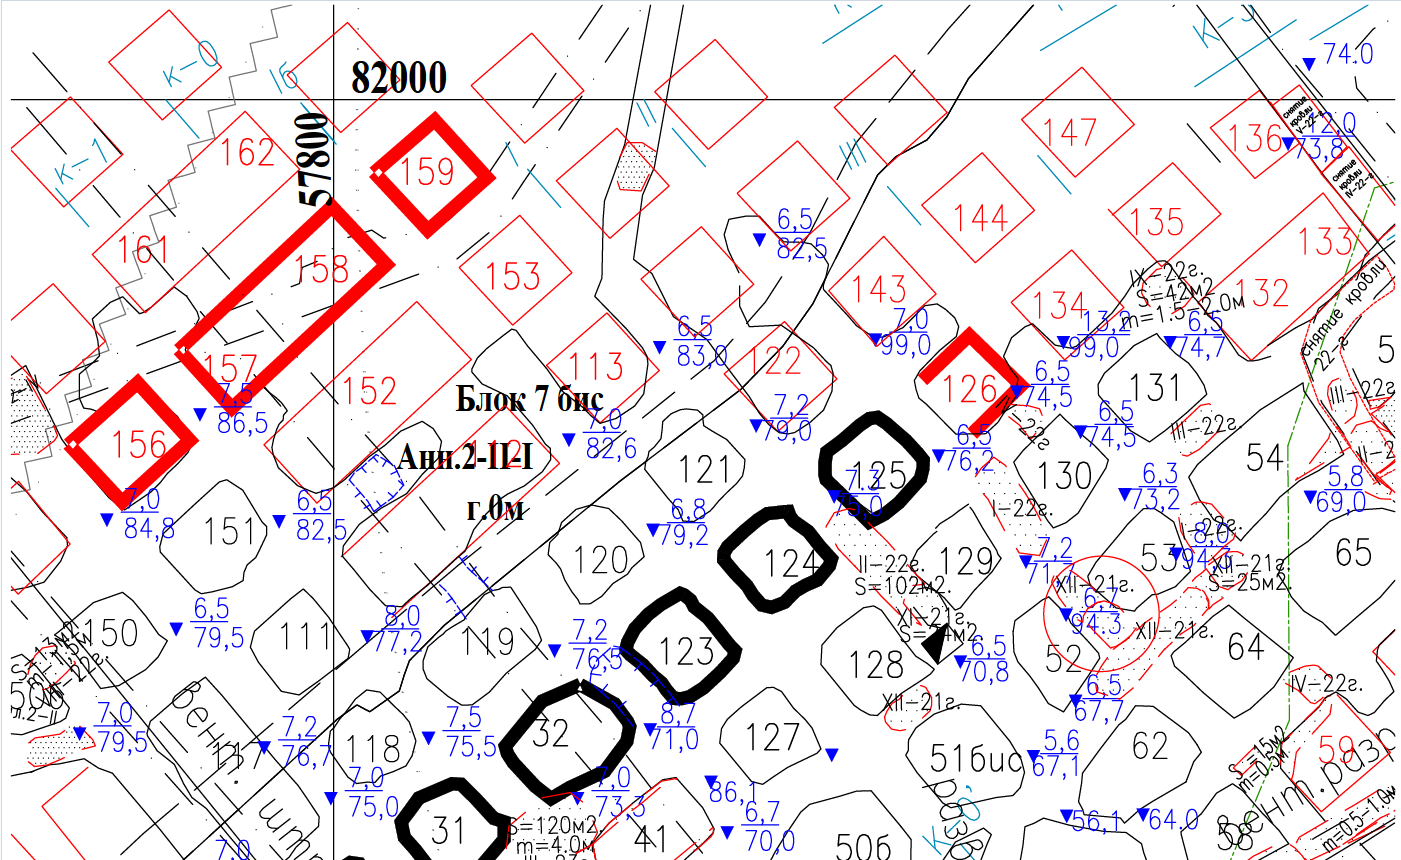
\includegraphics[width=0.6\textwidth]{media/gor/image9}
	\caption*{ Рис. 5 - Расположение испытуемых целиков в блоке 7 бис
	(156,157,158, 159)}
\end{figure}

\begin{figure}[H]
	\centering
	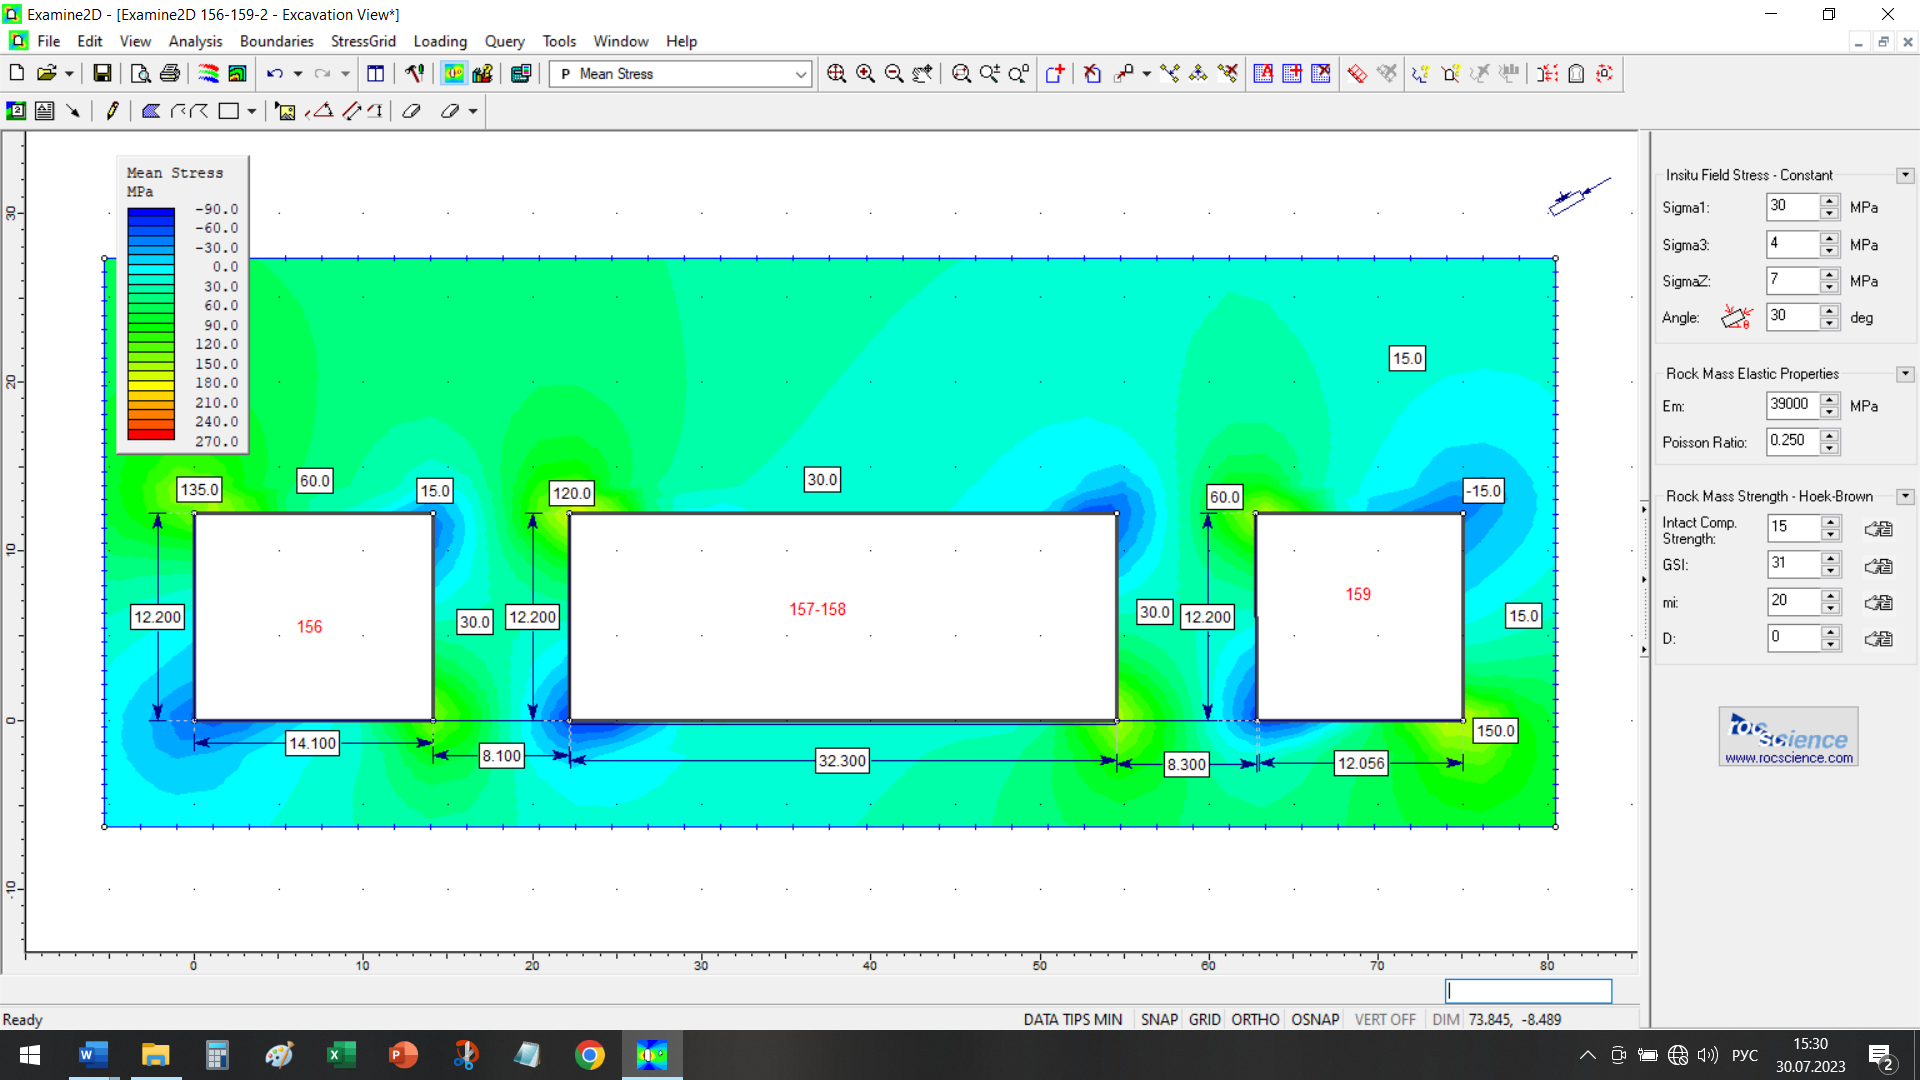
\includegraphics[width=0.6\textwidth]{media/gor/image10}
	\caption*{ Рис. 6 - Напряженно-деформированное состояние на 156, 157,
	158,159 целики, с учетом вертикальной нагрузки (вид сверху)}
\end{figure}

\begin{figure}[H]
	\centering
	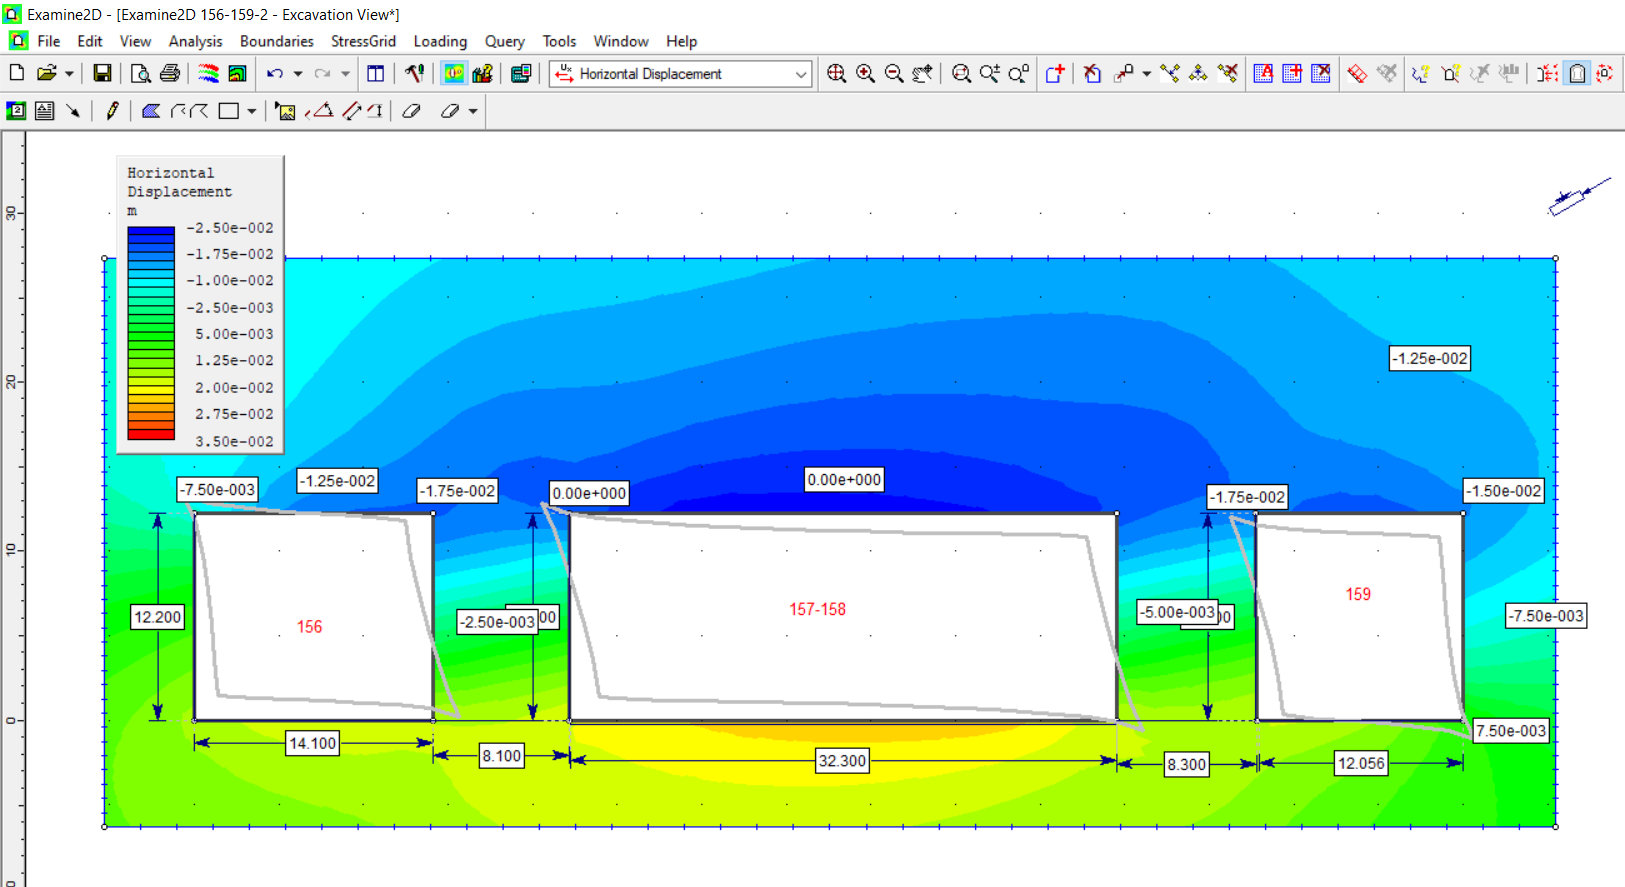
\includegraphics[width=0.6\textwidth]{media/gor/image11}
	\caption*{Рис. 7 - Напряженно-деформированное состояние на 156, 157,
	158,159 целики, с учетом горизонтального смещения (вид сверху)}
\end{figure}

\begin{figure}[H]
	\centering
	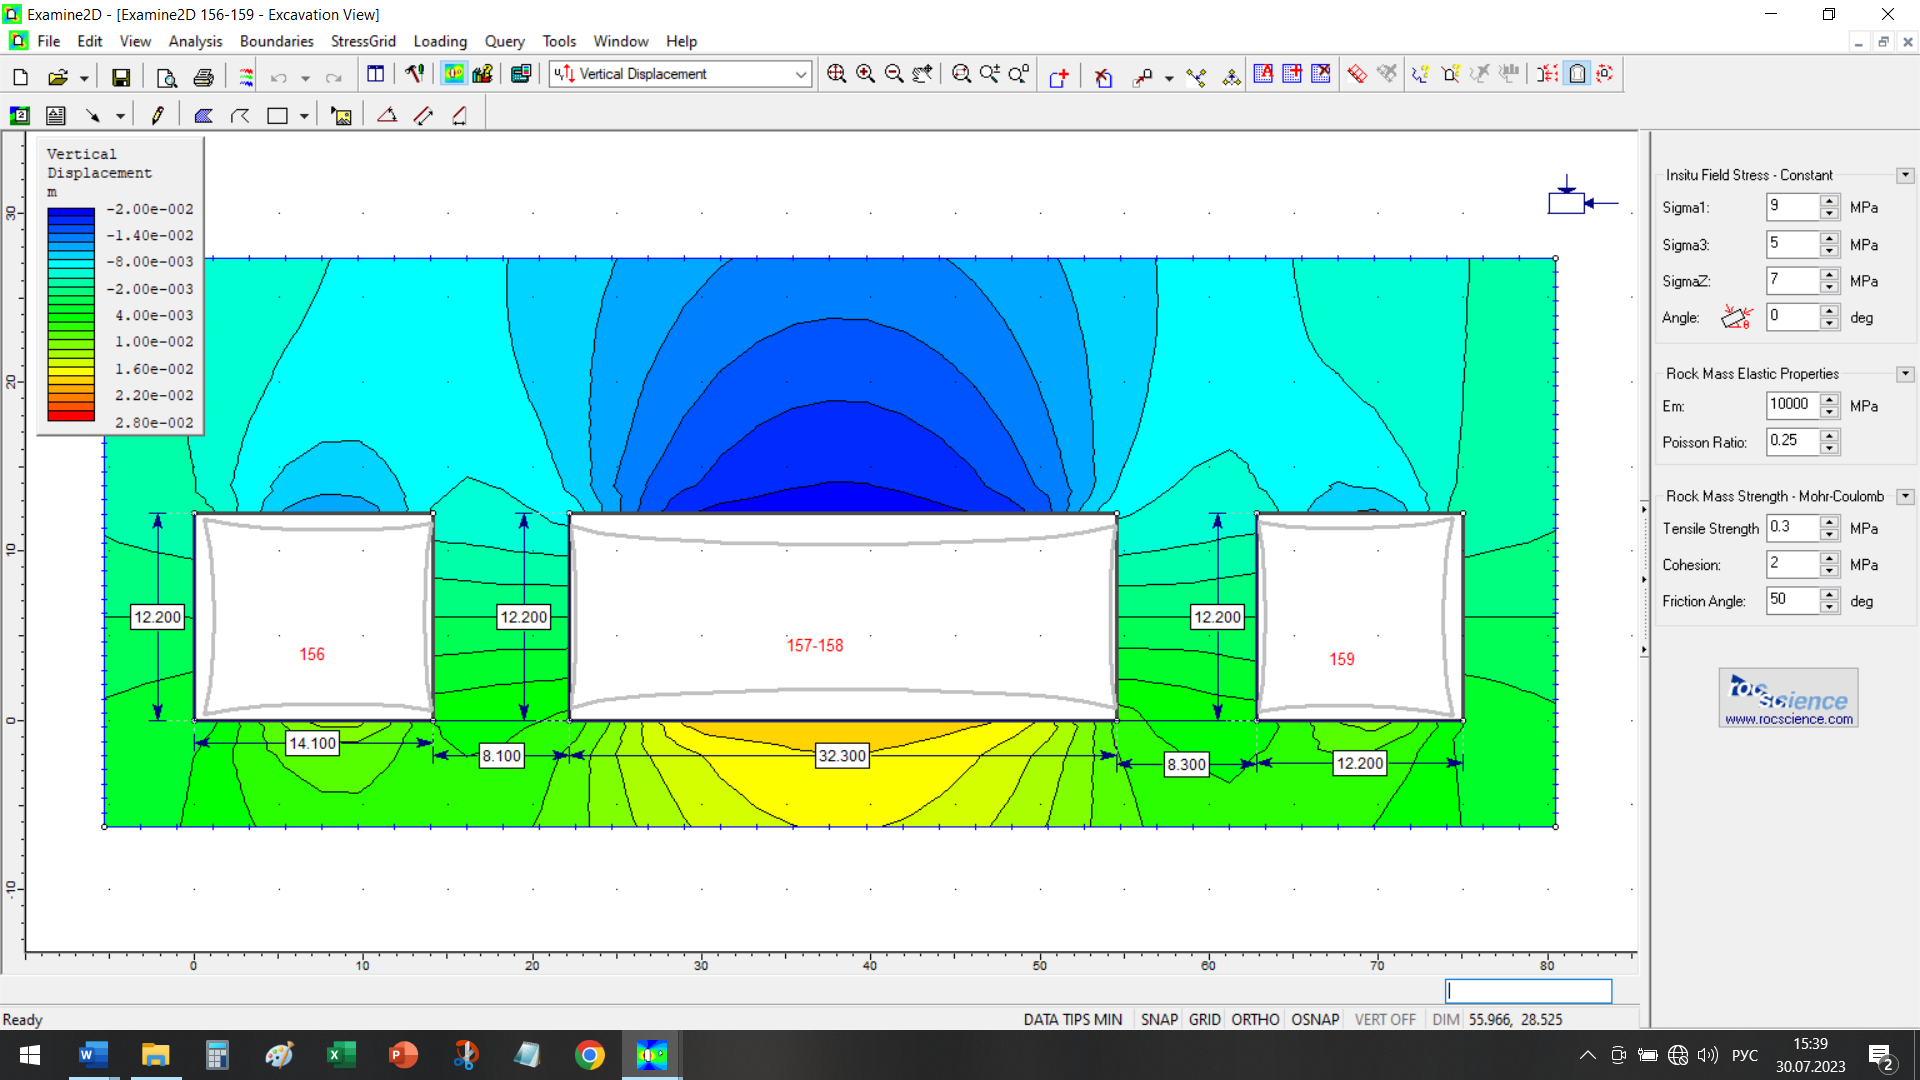
\includegraphics[width=0.6\textwidth]{media/gor/image12}
	\caption*{Рис. 8 - Напряженно-деформированное состояние на 156, 157,
	158,159 целики, с учетом вертикального смещения (вид сверху)}
\end{figure}

\begin{figure}[H]
	\centering
	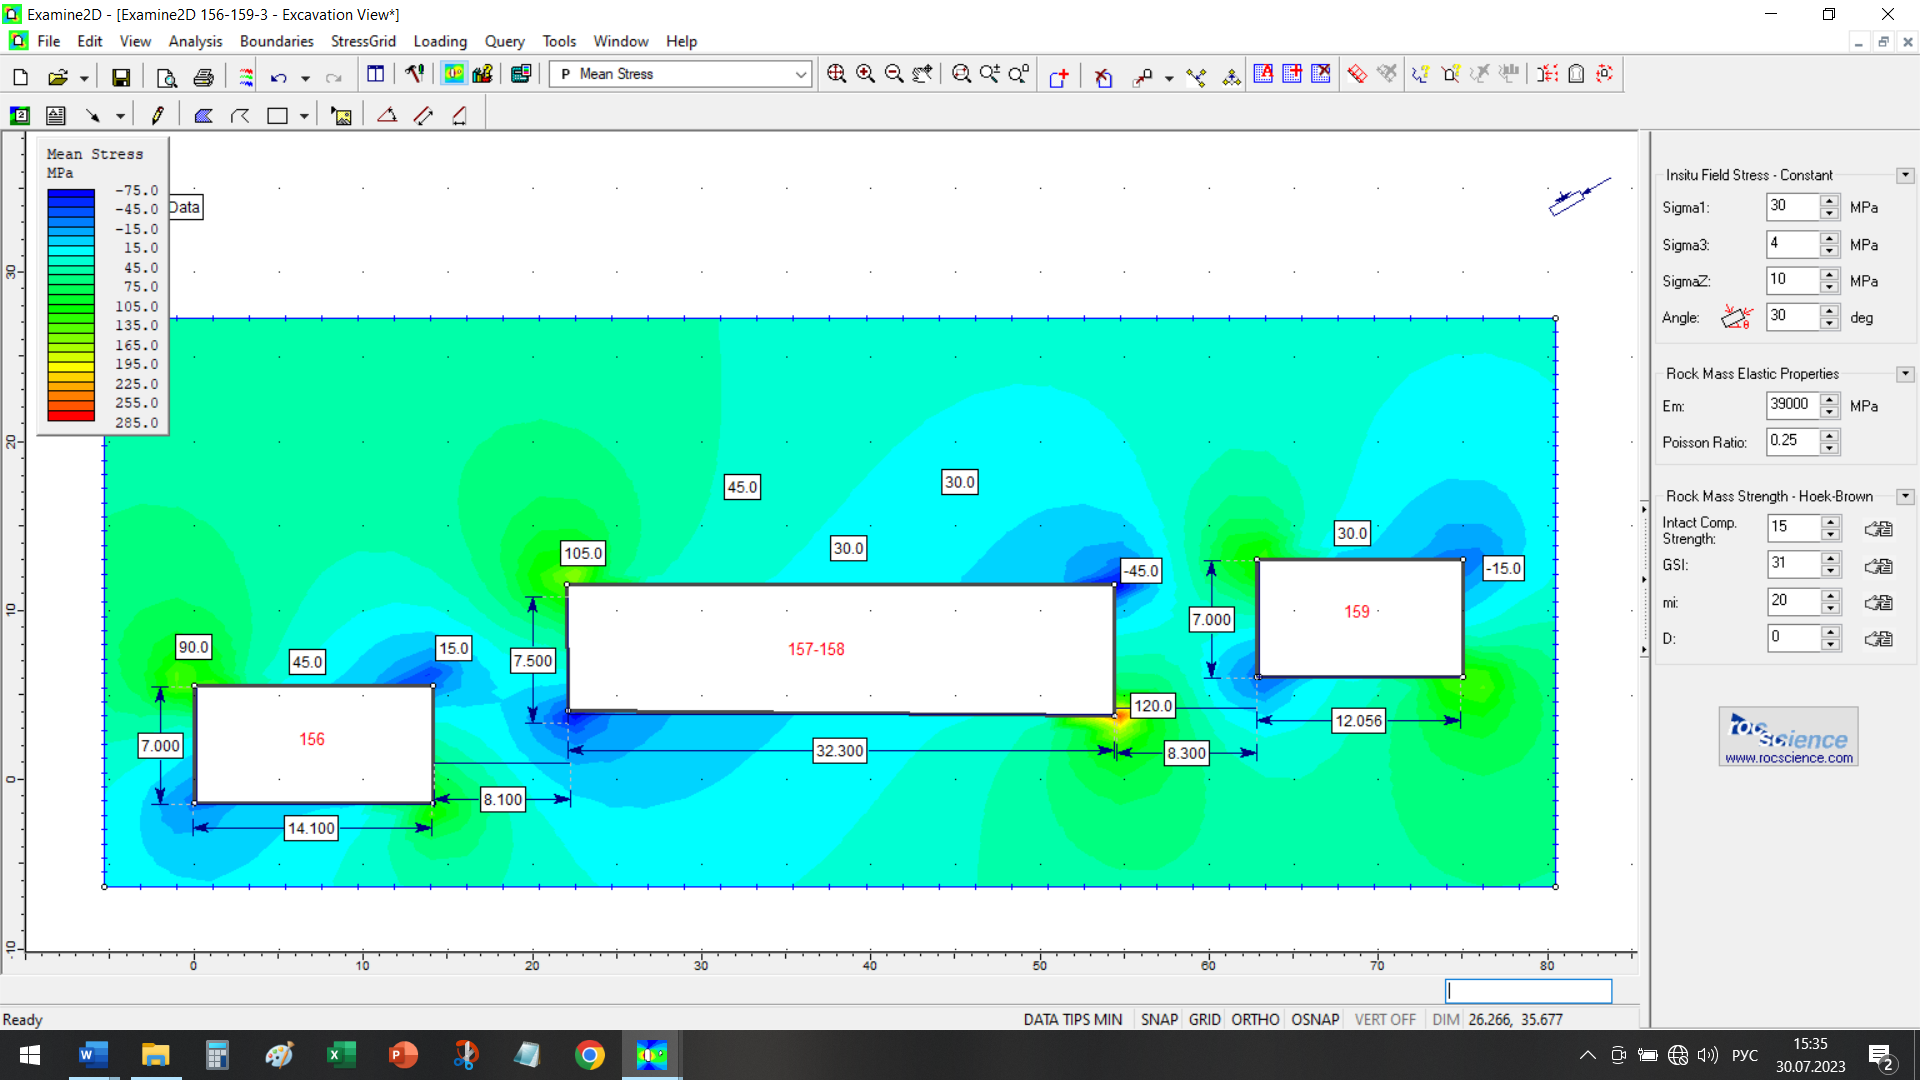
\includegraphics[width=0.6\textwidth]{media/gor/image13}
	\caption*{Рис. 9 - Напряженно-деформированное состояние на 156, 157,
	158,159 целики, с учетом вертикальной нагрузки (вид сбоку)}
\end{figure}

\begin{figure}[H]
	\centering
	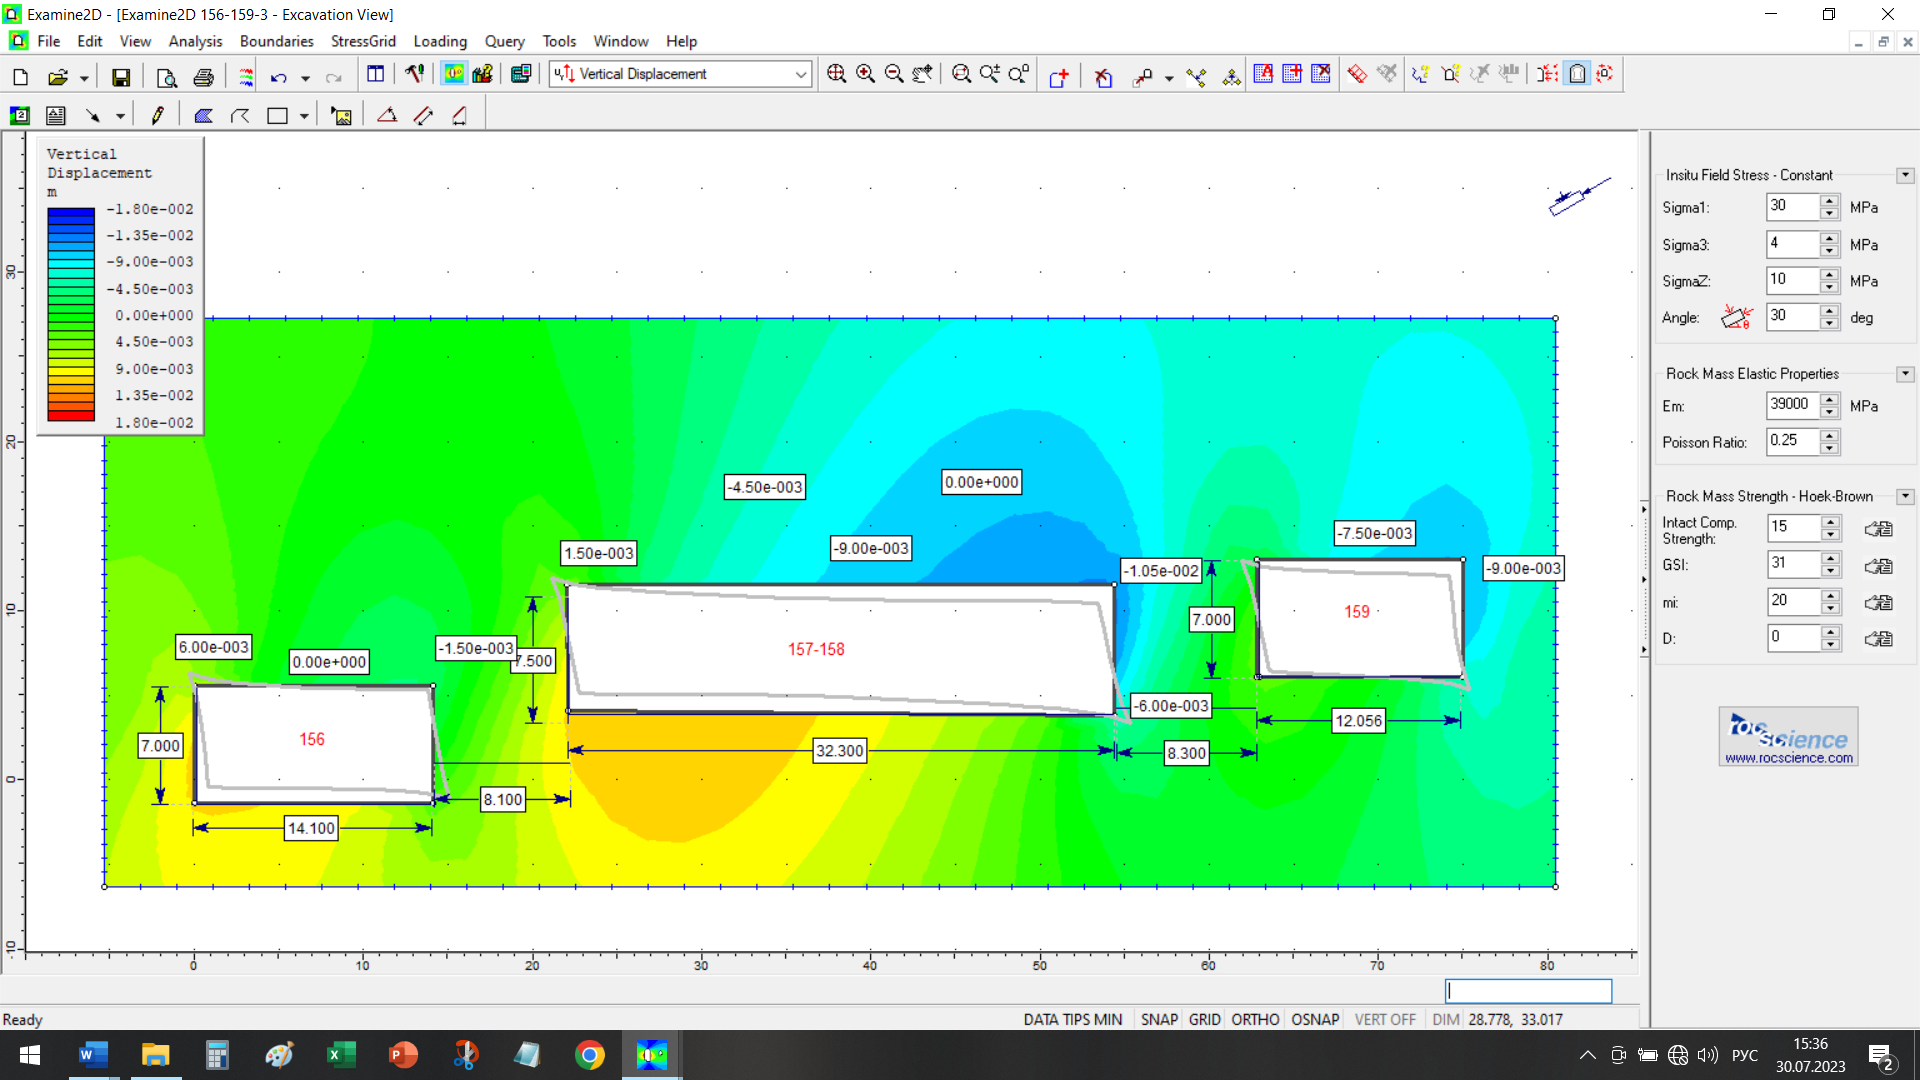
\includegraphics[width=0.6\textwidth]{media/gor/image14}
	\caption*{Рис. 10 - Напряженно-деформированное состояние на 156, 157,
	158,159 целики, с учетом вертикального смещения (вид сбоку)}
\end{figure}

\begin{figure}[H]
	\centering
	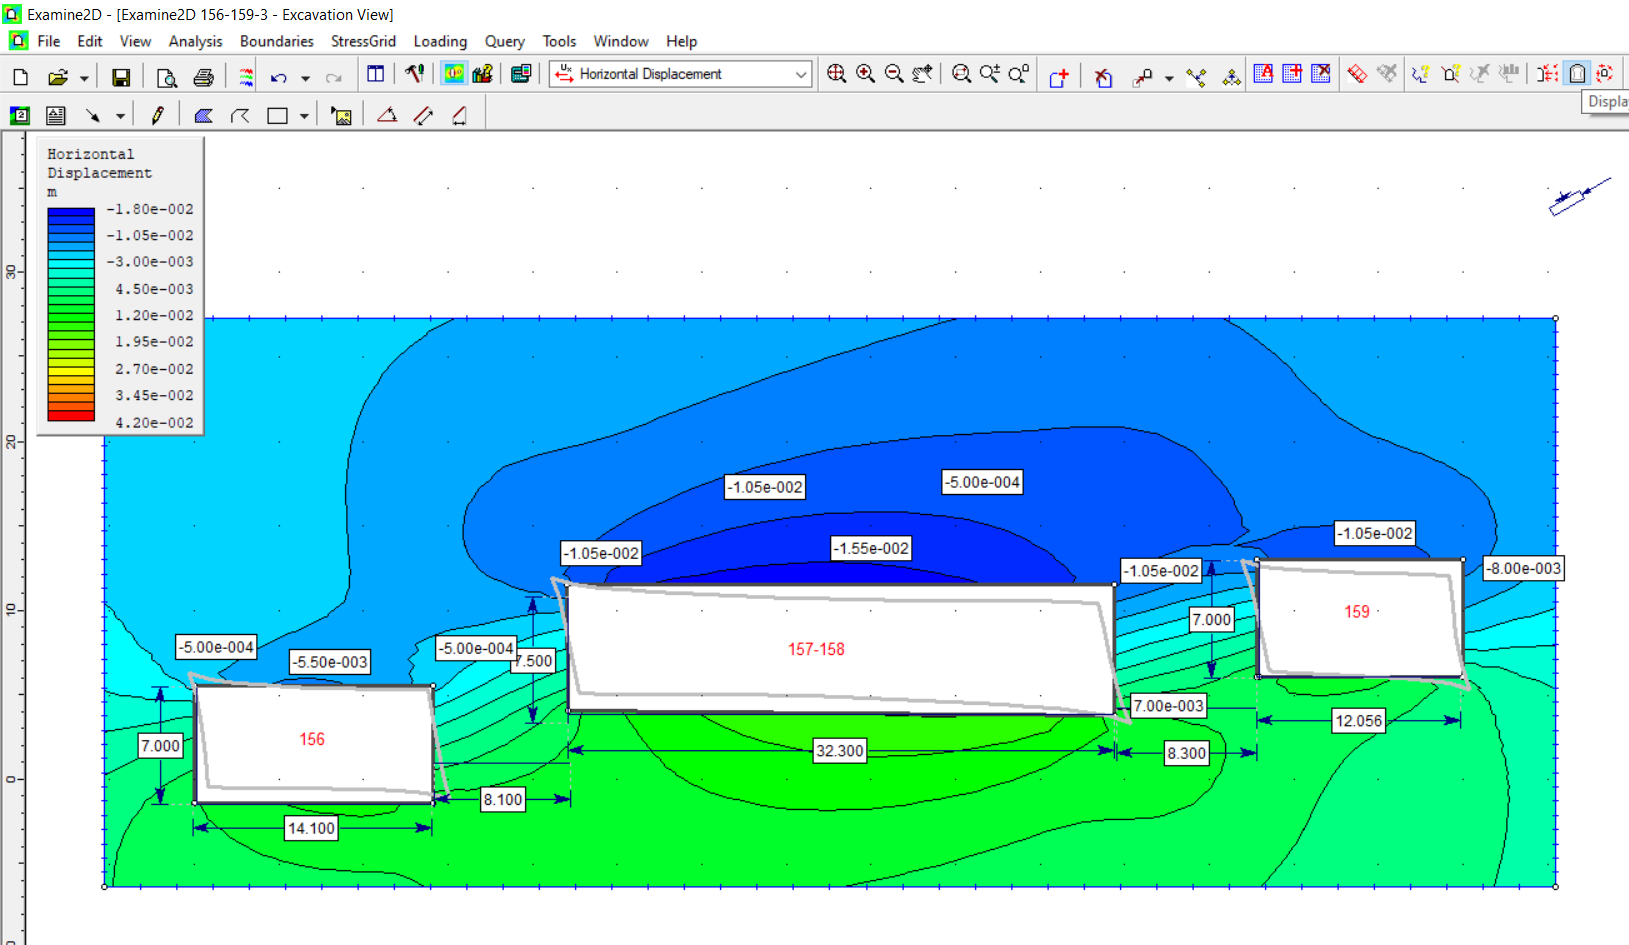
\includegraphics[width=0.6\textwidth]{media/gor/image15}
	\caption*{Рис. 11 - Напряженно-деформированное состояние на 156, 157,
	158,159 целики, с учетом горизонтального смещения (вид сбоку)}
\end{figure}

\begin{figure}[H]
	\centering
	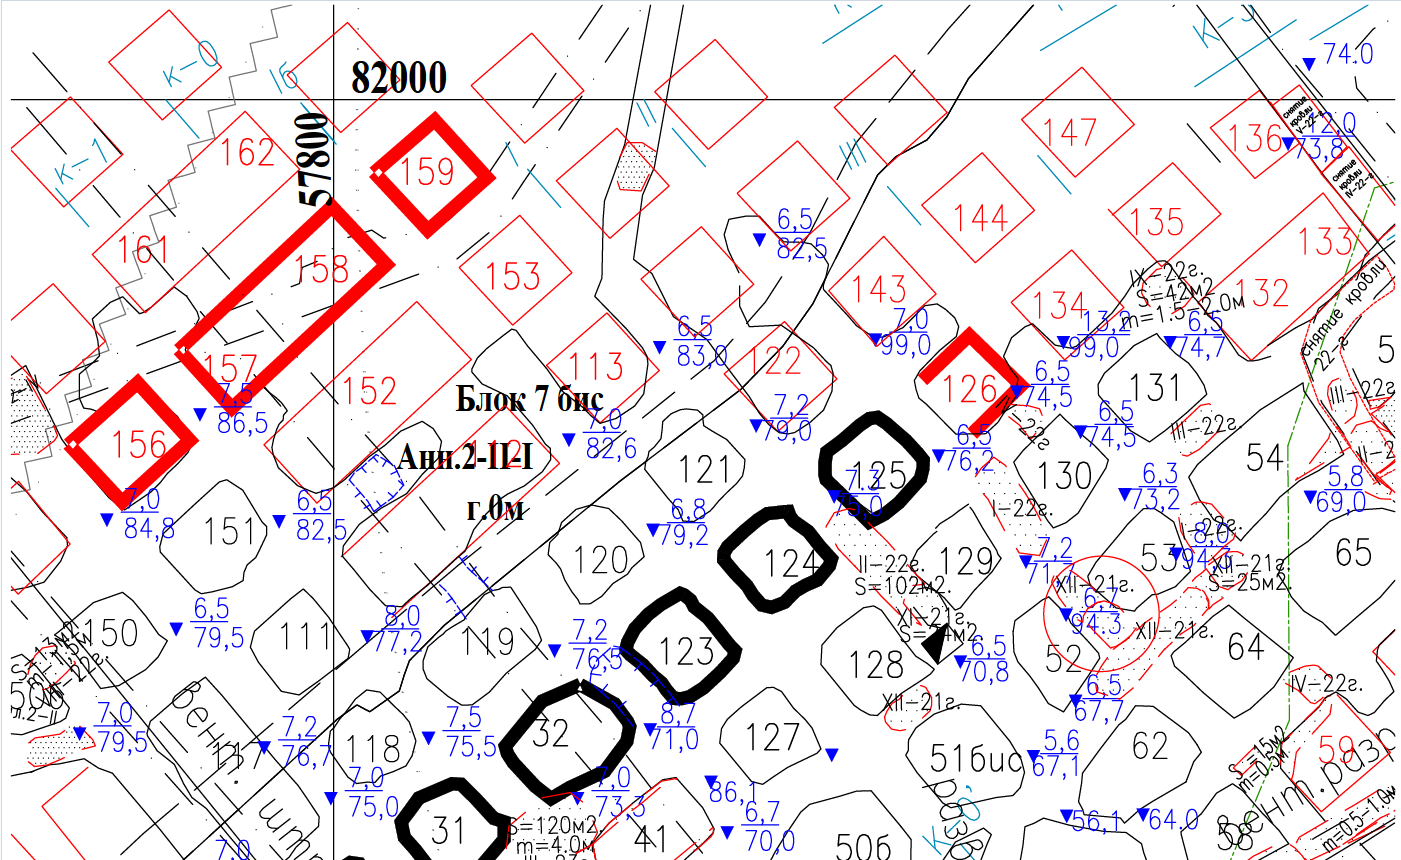
\includegraphics[width=0.6\textwidth]{media/gor/image9}
	\caption*{Рис. 12 - Расположение испытуемых целиков в блоке 7 бис
	(31-126)}
\end{figure}

\begin{figure}[H]
	\centering
	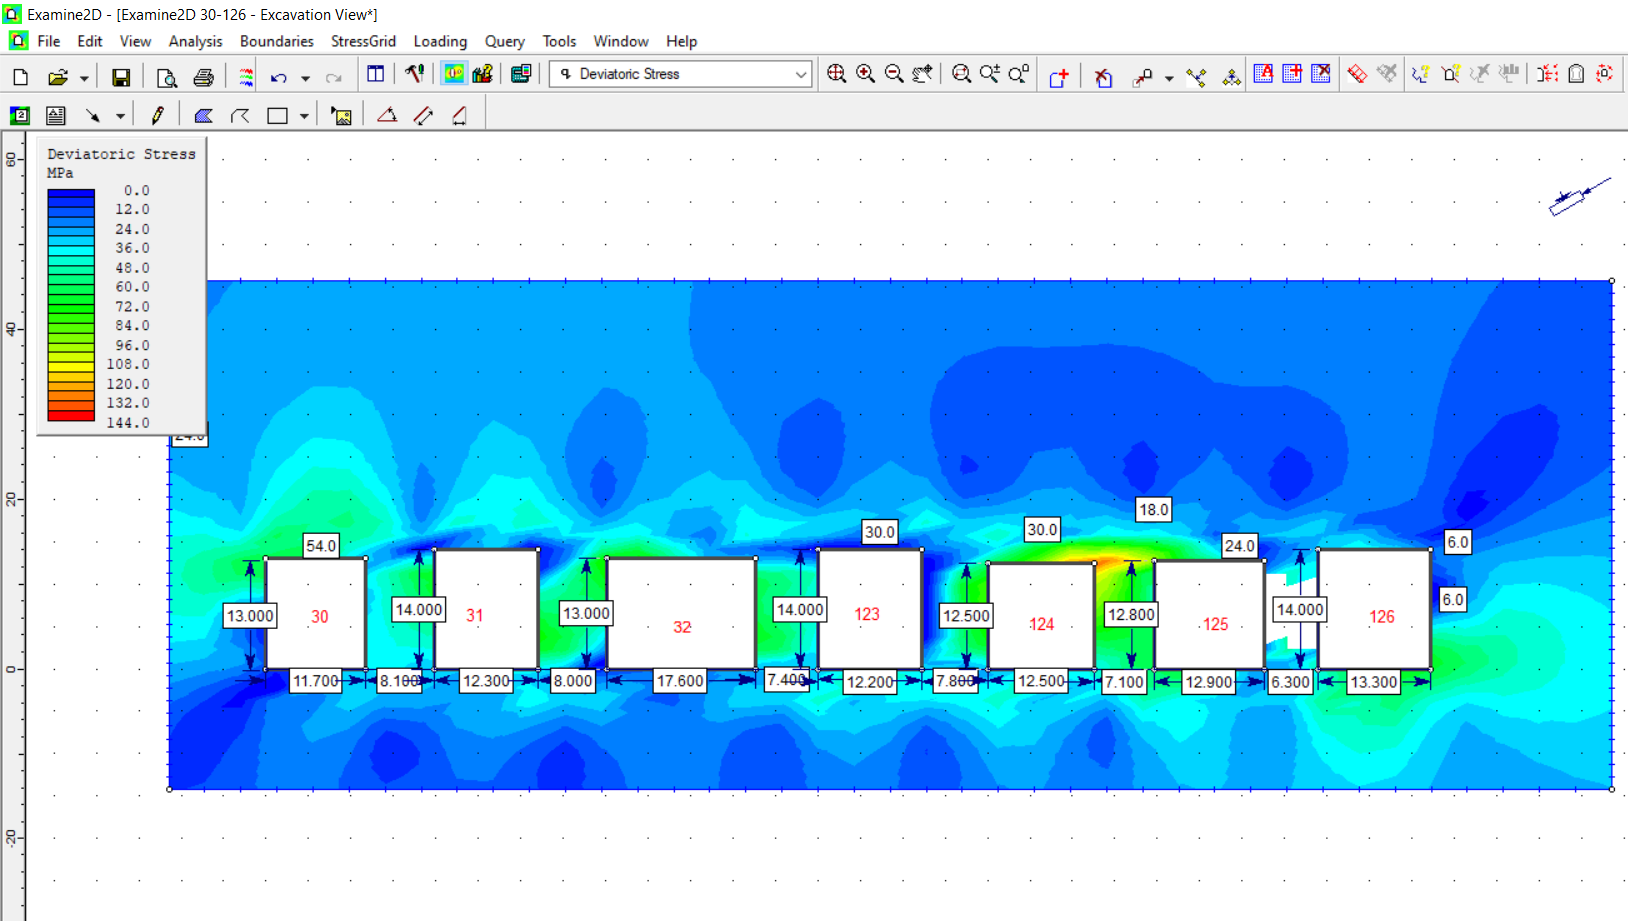
\includegraphics[width=0.6\textwidth]{media/gor/image16}
	\caption*{Рис. 13 - Напряженно-деформированное состояние на 30, 31,
	32,123, 124, 125, 126 целики, с учетом вертикальной нагрузки (вид сверху)}
\end{figure}

\begin{figure}[H]
	\centering
	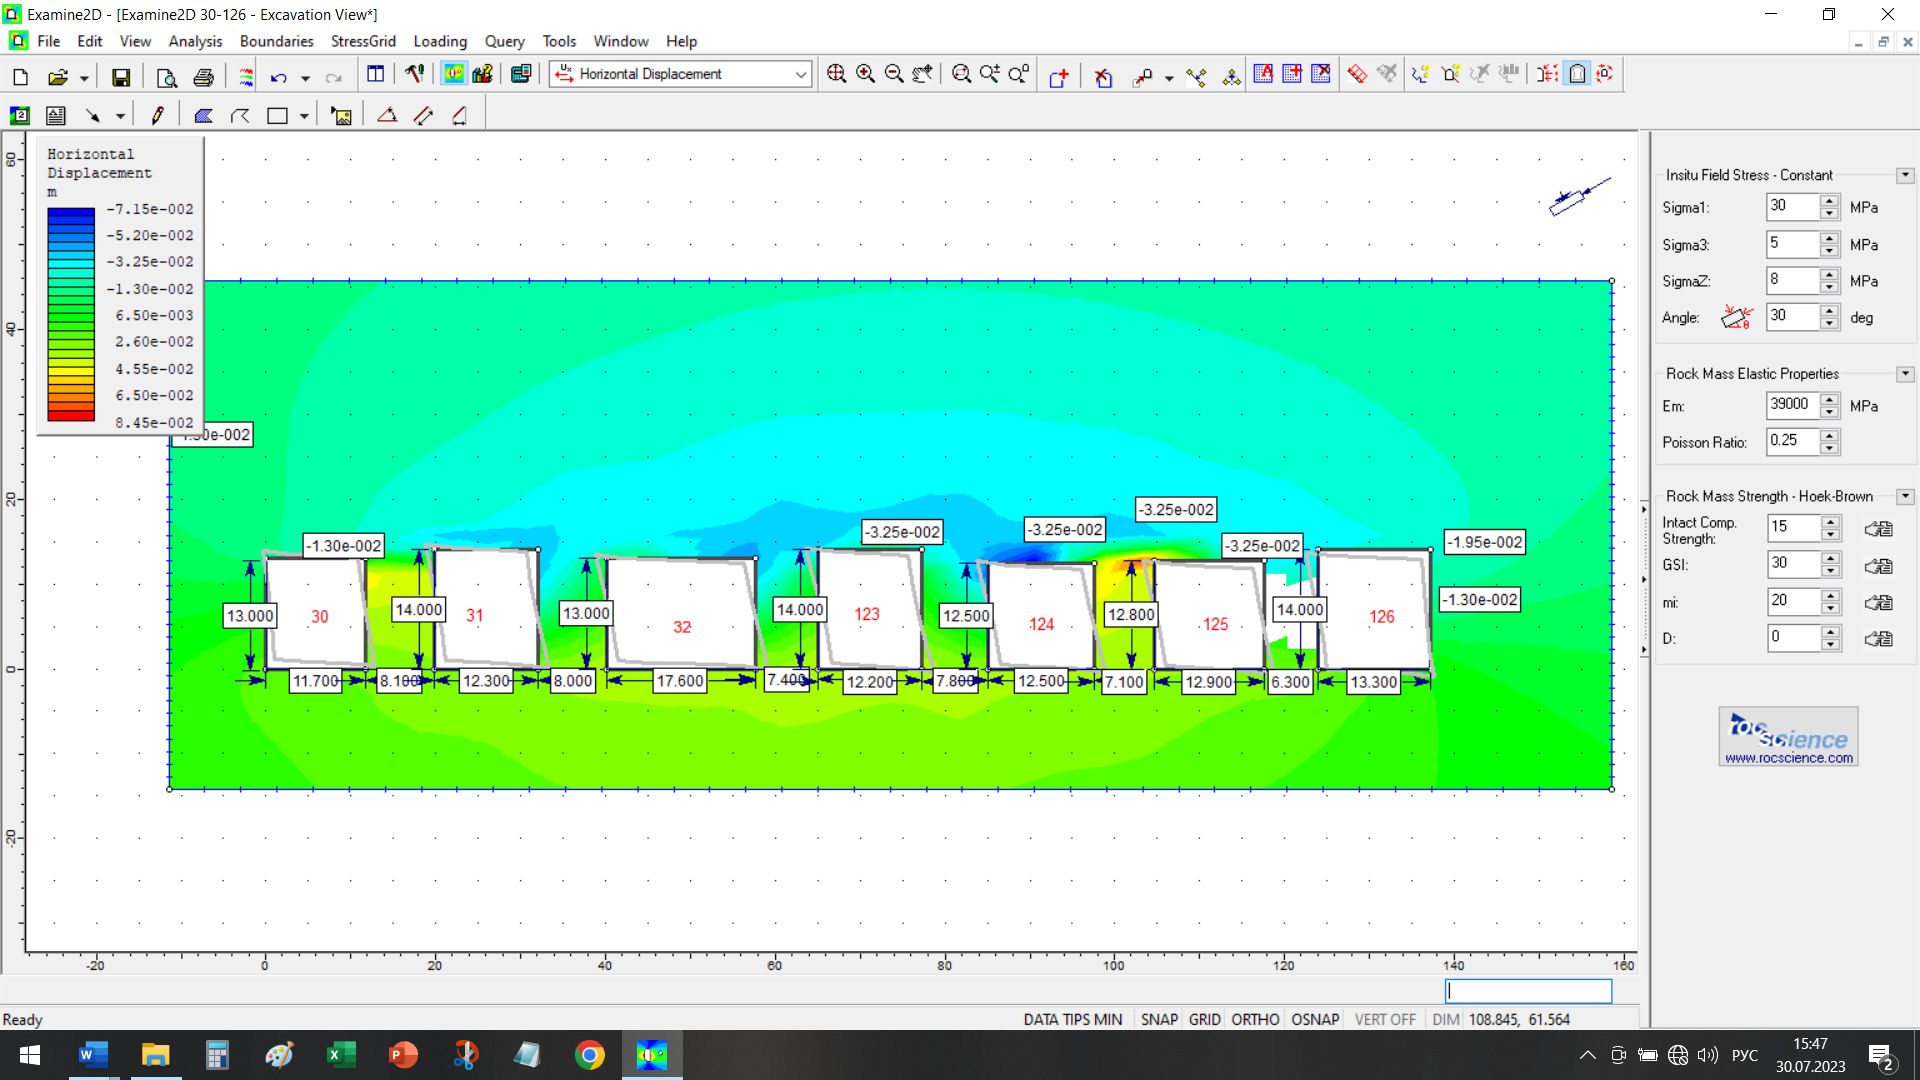
\includegraphics[width=0.6\textwidth]{media/gor/image17}
	\caption*{Рис. 14 - Напряженно-деформированное состояние на 30, 31,
	32,123, 124, 125, 126 целики, с учетом вертикального смещения (вид сверху)}
\end{figure}

\begin{figure}[H]
	\centering
	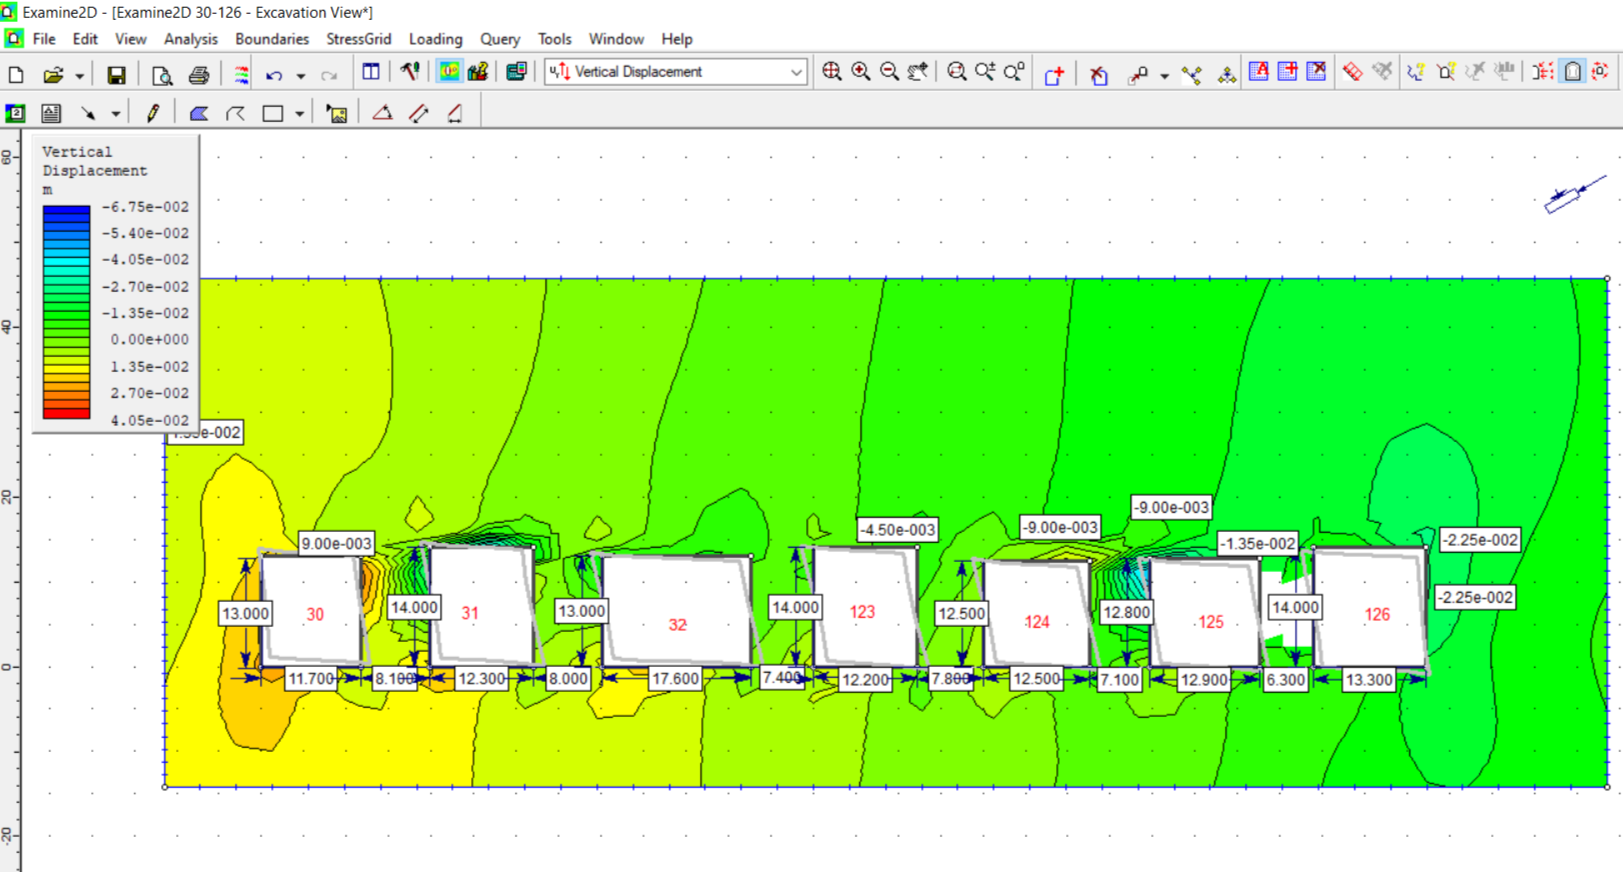
\includegraphics[width=0.6\textwidth]{media/gor/image18}
	\caption*{Рис. 15 - Напряженно-деформированное состояние на 30, 31,
	32,123, 124, 125, 126 целики, с учетом горизонтального смещения (вид сверху)}
\end{figure}

\begin{figure}[H]
	\centering
	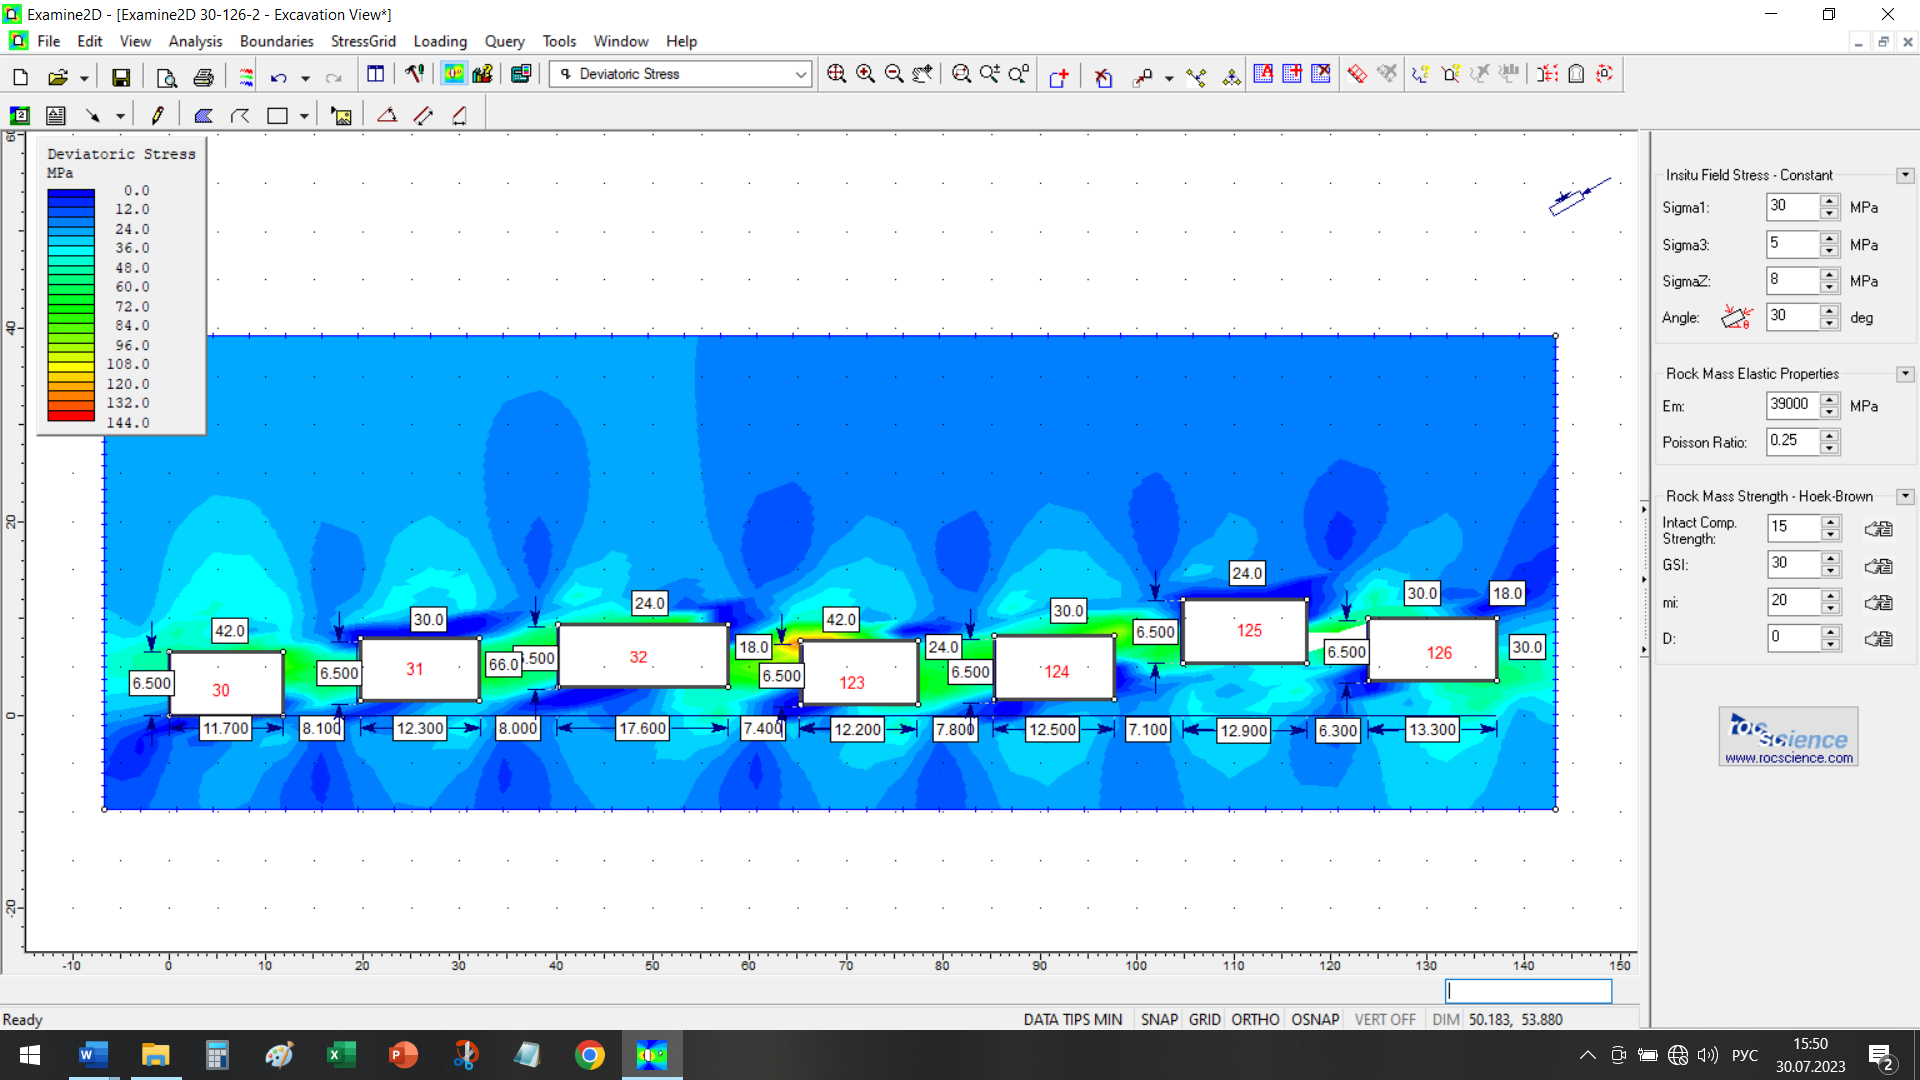
\includegraphics[width=0.6\textwidth]{media/gor/image19}
	\caption*{Рис. 16 - Напряженно-деформированное состояние на 30, 31,
	32,123, 124, 125, 126 целики, с учетом вертикальной нагрузки (вид сбоку)}
\end{figure}

\begin{figure}[H]
	\centering
	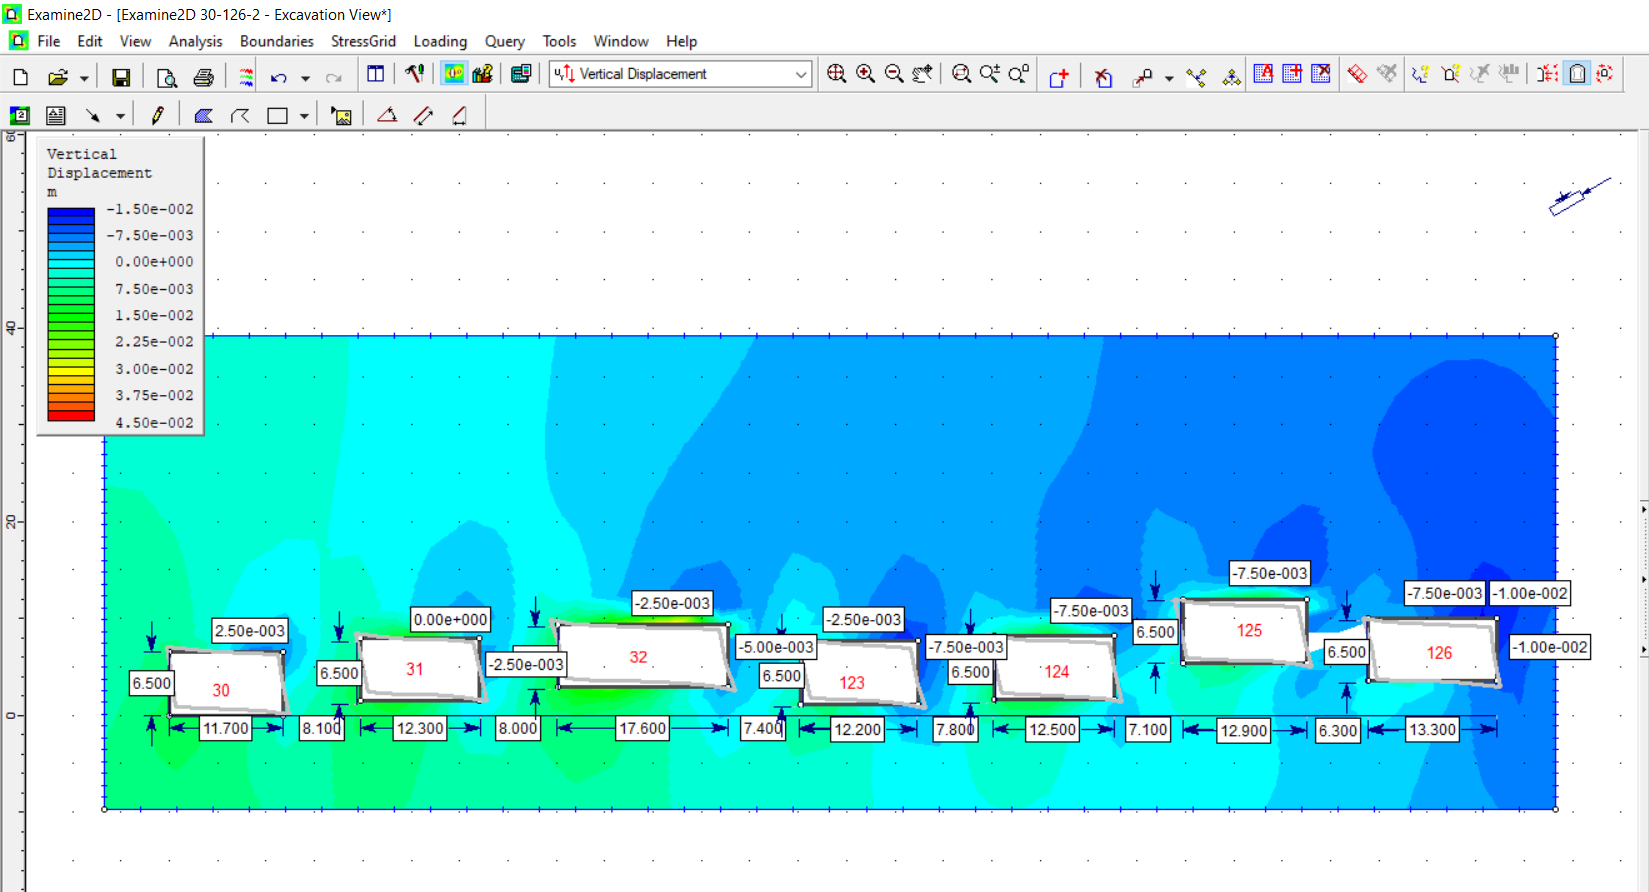
\includegraphics[width=0.6\textwidth]{media/gor/image20}
	\caption*{Рис. 17 - Напряженно-деформированное состояние на 30, 31,
	32,123, 124, 125, 126 целики, с учетом вертикального смещения (вид сбоку)}
\end{figure}

\begin{figure}[H]
	\centering
	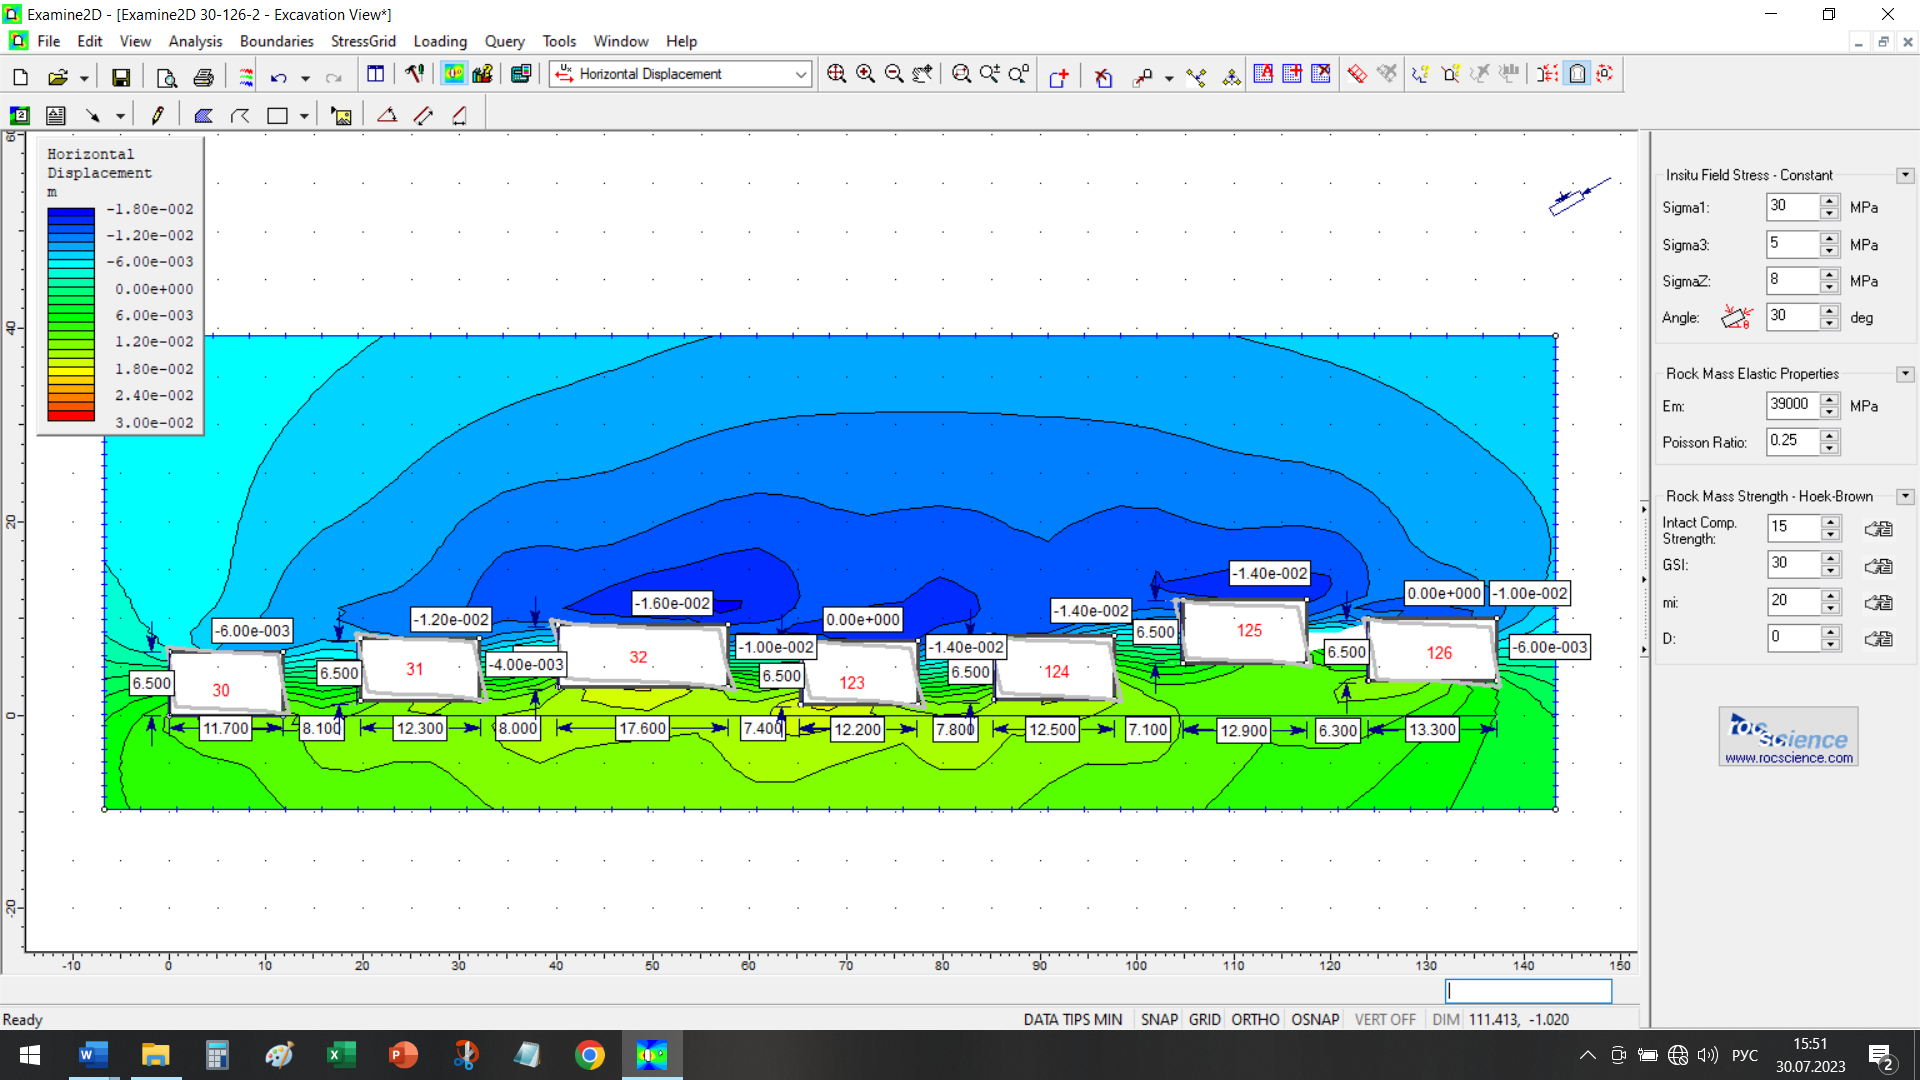
\includegraphics[width=0.6\textwidth]{media/gor/image21}
	\caption*{Рис. 18 - Напряженно-деформированное состояние на 30, 31,
	32,123, 124, 125, 126 целики, с учетом горизонтального смещения (вид сбоку)}
\end{figure}

\begin{multicols}{2}
По результатам численного моделирования действующих напряжений был
проведен расчет в соответствии свойствам для красноцветных пород,
который включает:

- предел прочности на одноосное сжатие 85 МПа;

- предел прочности на растяжение 6,5МПа.

Обрушения наклонной выработки проявляются в разы больше расположенных в
вышележащих целиках (верхних целиках) и представлены на рисунках 13 -
18. По результатам расчетов на соответствующие нагрузки на МКЦ при
глубине разработки 300, 400, 500, 600 метров проявляются деформации в
виде вертикального смещения на целиках, влияющие на их несущую
способность. К примеру, нагрузка равная 750т/м\textsuperscript{2} при
глубине разработки наклонных залежей H=300м, смещение массива в МКЦ
высотой h=10м расчетное значение на нижних целиках равно 4,5 м, а в
верхних целиках примерно 6,8 метров (таблица 1). Соответственно, разница
в напряжениях и их перемещениях между верхними и нижними целиками равна
до 50\%. Максимальное перемещение различных нагрузок при выемке руды
относительно глубины разработки показано в таблице 2.
\end{multicols}

\begin{table}[H]
\caption*{Таблица 2 - Максимальное перемещение различных нагрузок при
выемке руды}
\centering
\begin{tabular}{|c|c|c|cc|c|}
\hline
\multirow{2}{*}{№} &
  \multirow{2}{*}{\begin{tabular}[c]{@{}c@{}}Глубина\\ (м)\end{tabular}} &
  \multirow{2}{*}{\begin{tabular}[c]{@{}c@{}}Давление\\ P=γ·H\\  γ = 2.5т/м3\end{tabular}} &
  \multicolumn{2}{p{0.3\textwidth}|}{Максимальное перемещение по вертикали в (м) при выемке} &
  \multirow{2}{*}{Примечание} \\ \cline{4-5}
  &     &           & \multicolumn{1}{p{0.15\textwidth}|}{на верхних целиках (м)} & \multicolumn{1}{p{0.15\textwidth}|}{на нижних целиках (м)} & \\ \hline
1 &
  300 &
  750 т/м2 &
  \multicolumn{1}{c|}{-6,8} &
  -4,5 &
  \begin{tabular}[c]{@{}c@{}}Сильное обрушение \\ верних целиков, потеря \\ целостности нижних целиков\end{tabular} \\ \hline
2 & 400 & 1000 т/м2 & \multicolumn{1}{c|}{-8,3}                   & -5,4                  & Полное обрушение всех целиков \\ \hline
3 & 500 & 1250 т/м2 & \multicolumn{1}{c|}{-9,8}                   & -6,35                 & -                             \\ \hline
4 & 600 & 1500 т/м2 & \multicolumn{1}{c|}{-11,4}                  & -7,3                  & -                             \\ \hline
\end{tabular}%
\end{table}

\begin{multicols}{2}
{\bfseries Выводы.} Проведен расчетный анализ геомеханической ситуации
напряженно-дефрмированного состояния оставленного МКЦ в очистном
пространстве камерно-столбовой системы наклонных залежей под углом 20º с
применением метода конечных элементов в условиях обрушенной зоны с
мульдой сдвижения на примере шахты «Анненская» ВЖР:

- расчет вариантов систем разработки реализован с применением метода
конечных элементов в программе RS Examine2D с двухмерным моделированием
методом граничных элементов напряженно-деформированного состояния
массива при подземной разработке в упругой постановке, где данная
программа является интерактивной и простой в использовании, идеально
подходит для осуществления быстрого параметрического анализа для
предварительного проектирования, а также в качестве обучающего средства
численному анализу напряжений в геотехнических задачах;

- по результатам численного моделирования действующих напряжений был
проведен расчет в соответствии свойствам для красноцветных пород,
который составляет:

- предел прочности на одноосное сжатие 85 МПа;

- предел прочности на растяжение 6,5 МПа.

По результатам расчетов на соответствующие нагрузки на МКЦ при глубине
разработки 300, 400, 500, 600 метров проявляются деформации в виде
вертикального смещения на целиках, влияющие на их несущую способность.
\end{multicols}

\begin{center}
{\bfseries Литература}
\end{center}
\begin{references}

1. Технико-экономическое обоснование «Генеральный план разработки
месторождения Жезказган», том 6, Предварительные исследования и
предложения по направлениям разработки и порядку проведения подземных
горных работ» (Пояснительная записка) П13-19/05, Головной проектный
институт ТОО „Корпорация Казахмыс``, 2013. - 114 с.

2.Методические рекомендации по подземной отработке запасов пологих и
наклонных рудных залежей жезказганского месторождения, в том числе в
районах, примыкающих к ослабленным и обрушенным участкам. ИГД им. Д.А.
Кунаева» ПО "Жезказганцветмет» ТОО "Корпорация Казахмыс». Алматы --
Жезказган, 2010. - 122 с.

3. Презентационный доклад генерального директора Государственной
горнодобывающей компании ТОО «Корпорация Казахмыс» Кыркпышева Б. // IV
международная научно-практическая конференция «Геотехника-2013»:
Проблемы и пути инновационного развития горной промышленности. - Алматы.
-- 2013.

4. Итоговый отчет за 2022 год по теме НИР «Исследование соответствия
определения параметров и системы разработки в условиях шахты
„Анненская`` Восточно-Жезказганского рудника». Руководитель проекта
Бекбергенов Д.К., ТОО «КазНИИЦветмет». Алматы, 2022. - 347 с.

5. Руководство по проектированию разработки наклонных залежей
Жезказганского месторождения. Корпорация «Казахмыс»,
«ЖезказганНИПИцветмет», ИГД им. Д.А. Кунаева, 2002.- 50 с.

6. Аханов Т.М. Создание высокоэффективных технологий разработки
месторождений в условиях подземных рудников ТОО «Корпорация Казахмыс» //
Горный журнал Казахстана.-2009, № 11.- С.26-30

7. Герасименко В.И., Макаров А.Б., Зотеев О.В. Анализ геомеханического
состояния выработанных пространств Жезказганского месторождения. Часть
1. ГГУ ТОО «Корпорация Казахмыс», Караганда-Жезказган, 2010. - 52 с.

8. Аханов Т.М., Прокушев Г.А. Технология разработки Жезказганского
месторождения, состояние и перспективы развития. Горный журнал
Казахстана, №1(57), 2010. - с.12-17

9.Бекбергенов Д.К. О повторной подземной отработке технологии с
самообрушением руды с высокой полнотой извлечения запасов на обрушенных
и ослабленных участках Жезказгана // Тезисы докладов Международной
научно-практической конференции «Горное дело и металлургия в Казахстане.
Состояние и перспективы», посвященной 100-летию со дня рождения
академика Байконурова Омирхана Аймаганбетовича, 11-12 октября 2012 г.,
КазНТУ. - Алматы. - 2012. - С. 52-55

10. Методы определения размеров несущих колонн и перекрытий. Москва:
Изд. АН СССР, 1962. - 199 с.

11. Ковальчук О.А., Колесников А.В., Русанова Е.М. Введение в
программный комплекс ЛИРА 10.4. учебное пособие. Москва, 2015 г. -185 с.

12. Либерман Ю.М., Гомес Ц. Метод определения давления на целик при
разработке изолированными панелями. В сб."Физико-механические свойства,
давление и разрушение горных пород", М., АН СССР, 1962.- С. 133 - 140
\end{references}

\begin{center}
{\bfseries References}
\end{center}

\begin{references}

1. Tehniko-jekonomicheskoe obosnovanie «General' nyj plan
razrabotki mestorozhdenija Zhezkazgan», tom 6,
Predvaritel' nye issledovanija i predlozhenija po
napravlenijam razrabotki i porjadku provedenija podzemnyh gornyh rabot»
(Pojasnitel' naja zapiska) P13-19/05, Golovnoj proektnyj
institut TOO „Korporacija Kazahmys``, 2013. - 114 s. {[}Russian{]}

2.Metodicheskie rekomendacii po podzemnoj otrabotke zapasov pologih i
naklonnyh rudnyh zalezhej zhezkazganskogo mestorozhdenija, v tom chisle
v rajonah, primykajushhih k oslablennym i obrushennym uchastkam. IGD im.
D.A. Kunaeva» PO "Zhezkazgancvetmet» TOO "Korporacija Kazahmys». Almaty
-- Zhezkazgan, 2010. - 122 s. {[}Russian{]}

3. Prezentacionnyj doklad general' nogo direktora
Gosudarstvennoj gornodobyvajushhej kompanii TOO \\«Korporacija Kazahmys»
Kyrkpysheva B. // IV mezhdunarodnaja nauchno-prakticheskaja konferencija
«Geotehnika-2013»: Problemy i puti innovacionnogo razvitija gornoj
promyshlennosti. - Almaty.- 2013. {[}Russian{]}

4. Itogovyj otchet za 2022 god po teme NIR «Issledovanie sootvetstvija
opredelenija parametrov i sistemy razrabotki v uslovijah shahty
„Annenskaja`` Vostochno-Zhezkazganskogo rudnika».
Rukovoditel'{} proekta Bekbergenov D.K., TOO
«KazNIICvetmet». Almaty, 2022. - 347 s. {[}Russian{]}

5.Rukovodstvo po proektirovaniju razrabotki naklonnyh zalezhej
Zhezkazganskogo mestorozhdenija.\\ Korporacija «Kazahmys»,
«ZhezkazganNIPIcvetmet», IGD im. D.A. Kunaeva, 2002.- 50 s.
{[}Russian{]}

6. Ahanov T.M. Sozdanie vysokojeffektivnyh tehnologij razrabotki
mestorozhdenij v uslovijah podzemnyh rudnikov TOO «Korporacija Kazahmys»
// Gornyj zhurnal Kazahstana.-2009, № 11.- S.26-30. {[}Russian{]}

7.Gerasimenko V.I., Makarov A.B., Zoteev O.V. Analiz geomehanicheskogo
sostojanija vyrabotannyh prostranstv Zhezkazganskogo mestorozhdenija.
Chast'{} 1. GGU TOO «Korporacija Kazahmys»,
Karaganda-Zhezkazgan, 2010. - 52 s. {[}Russian{]}

8.Ahanov T.M., Prokushev G.A. Tehnologija razrabotki Zhezkazganskogo
mestorozhdenija, sostojanie i perspektivy razvitija. Gornyj zhurnal
Kazahstana, №1(57), 2010. - s.12-17. {[}Russian{]}

9.Bekbergenov D.K. O povtornoj podzemnoj otrabotke tehnologii s
samoobrusheniem rudy s vysokoj polnotoj izvlechenija zapasov na
obrushennyh i oslablennyh uchastkah Zhezkazgana // Tezisy dokladov
Mezhdunarodnoj nauchno-prakticheskoj konferencii «Gornoe delo i
metallurgija v Kazahstane. Sostojanie i perspektivy», posvjashhennoj
100-letiju so dnja rozhdenija akademika Bajkonurova Omirhana

Ajmaganbetovicha, 11-12 oktjabrja 2012 g., KazNTU. - Almaty. - 2012. -
S. 52-55. {[}Russian{]}

10. Metody opredelenija razmerov nesushhih kolonn i perekrytij. Moskva:
Izd. AN SSSR, 1962. - 199 s. {[}Russian{]}

11. Koval' chuk O.A., Kolesnikov A.V., Rusanova E.M.
Vvedenie v programmnyj kompleks LIRA 10.4. uchebnoe posobie. Moskva,
2015 g. -185 s. {[}Russian{]}

12. Liberman Ju.M., Gomes C. Metod opredelenija davlenija na celik pri
razrabotke izolirovannymi \\paneljami. V sb."Fiziko-mehanicheskie
svojstva, davlenie i razrushenie gornyh porod", M., AN SSSR, 1962.- S.
133 -140. {[}Russian{]}
\end{references}

\begin{authorinfo}
\hspace{1em}\emph{{\bfseries Сведения об авторах}}

Савич И.Н.- доктор технических наук, профессоркафедры геотехнологии
освоения недр НИТУ МИСИС, Москва, Россия, е-mail: tpr\_msmu@mail.ru;

Бекбергенов Д.К.{\bfseries -}кандидат технических наук, заведующий
лабораторией «Комплексное освоение недр», Института горного дела имени
Д.А.Кунаева, Алматы, Казахстан, е-mail:
\href{mailto:kdbekbergen@mail.ru}{\nolinkurl{kdbekbergen@mail.ru}};

Зейнуллин А.А. {\bfseries --} д.т.н., профессор, АО «Казахский университет
технологии и бизнеса им.К.Кулажанова», Астана, Казахстан, е-mail:
\href{mailto:karim_57@mail.ru}{\nolinkurl{karim\_57@mail.ru}};

Жанакова Р.К. {\bfseries -} доктор PhD ассоциированный профессор Казахского
автомобильно- дорожного института имени Л.Б. Гончарова, е-mail:
\href{mailto:zhanakova_raisa@mail.ru}{\nolinkurl{zhanakova\_raisa@mail.ru}};

Сейтенов А.С. {\bfseries -} докторант Евразийского национального
университета им.Л.Н.Гумилева, Астана, Казахстан, \\е-mail:altynbekss@gmail.com;

Мейрам Д.Д.- докторант Карагандинского технического университета им.
А.Сагинова, АО «Казахский университет технологии и бизнеса
им.К.Кулажанова» Караганда, Астана, Казахстан,

е-mail:
\href{mailto:diana_meiram@mail.ru}{\nolinkurl{diana\_meiram@mail.ru}}

\hspace{1em}\emph{{\bfseries Information about the author}}

Savich I.N. - Doctor of Technical Sciences, Professor of the Department
of Geotechnology of Subsoil Development NUST MISIS, Moscow, Russia,
e-mail: tpr\_msmu@mail.ru;

Bekbergenov D.K. -- candidate of technical sciences, head of the
laboratory ``Complex development of subsoil'', Institute of Mining named
after D.A. Kunaev, Almaty, Kazakhstan, e-mail: kdbekbergen@mail.ru;

Zeinullin A.A. -- Doctor of Technical Sciences, Professor, JSC Kazakh
University of Technology and Business named after K. Kulazhanov, ,
Astana, Kazakhstan, e-mail: karim\_57@mail.ru

Zhanakova R.K. - Doctor PhD Associate Professor of the Kazakh Automobile
and Road Institute named after L.B. Goncharova, e-mail:zhanakova\_raisa@mail.ru;

Seitenov A.S. - doctoral student of the Eurasian National University
named after L.N. Gumilyov, Astana, Kazakhstan, e-mail: altynbekss@gmail.com

Meiram D.D. - doctoral student of A. Saginov Karaganda Technical
University, JSC Kazakh University of Technology and Business named after
K. Kulazhanov, Karaganda Astana, Kazakhstan,e-mail:
diana\_meiram@mail.ru
\end{authorinfo}
